\documentclass{article}

\usepackage[margin=1in]{geometry}
\usepackage{graphicx}
\usepackage{amsmath}
%\usepackage[noprefix]{nomencl}
%\usepackage[section]{placeins}
\usepackage[colorlinks,bookmarks,bookmarksnumbered,allcolors=blue]{hyperref}
%\usepackage{cite}
%\usepackage{doi}
%\usepackage[caption=false,justification=raggedright,singlelinecheck=false]{subfig}
%\usepackage{booktabs} % better tables
\usepackage[capitalise]{cleveref}
\usepackage{indentfirst}

\begin{document}

\author{Andrew Ning}
\title{Theory: Vortex Lattice Method}
% \date{August 3, 2017}
\maketitle

\section{Overview}

The vortex lattice method (VLM) is essentially an extension of thin airfoil theory into three dimensions.  It could also be thought of as a simplified implementation of a 3D panel code.  All potential theory is based on the assumption of irrotational flow: 
\begin{equation}
\nabla \times \vec{V} = 0
\end{equation}
This assumption allows us to express the velocity field in terms of a potential function:
\begin{equation}
\vec{V} = \nabla \phi
\end{equation}
If we also assume that the flow is incompressible:
\begin{equation}
\nabla \cdot \vec V = 0
\end{equation}
Then substituting in the vector potential yields Laplace's equation:
\begin{equation}
\nabla^2 \phi = 0
\end{equation}

Solutions are generally built up using singularities that already satisfy Laplace's equation and the boundary condition in the far-field.  In this case we use straight line vortex filaments.  A lifting surface is divided into panels, and each panel has a horseshoe vortex as shown in \cref{fig:horseshoe}, with the horse vortex extending into the $+x$ direction of the body axes.  

The first of Helmholtz' vortex theorems states that the vortex strength (and direction) must be constant throughout the horseshoe vortex.  The second theorem states that the vortex must form a closed path or end at the boundary.  We take the boundary infinitely far away and so can treat the vortex with three segments (hence the horseshoe name).  

\begin{figure}[htbp]
\centering
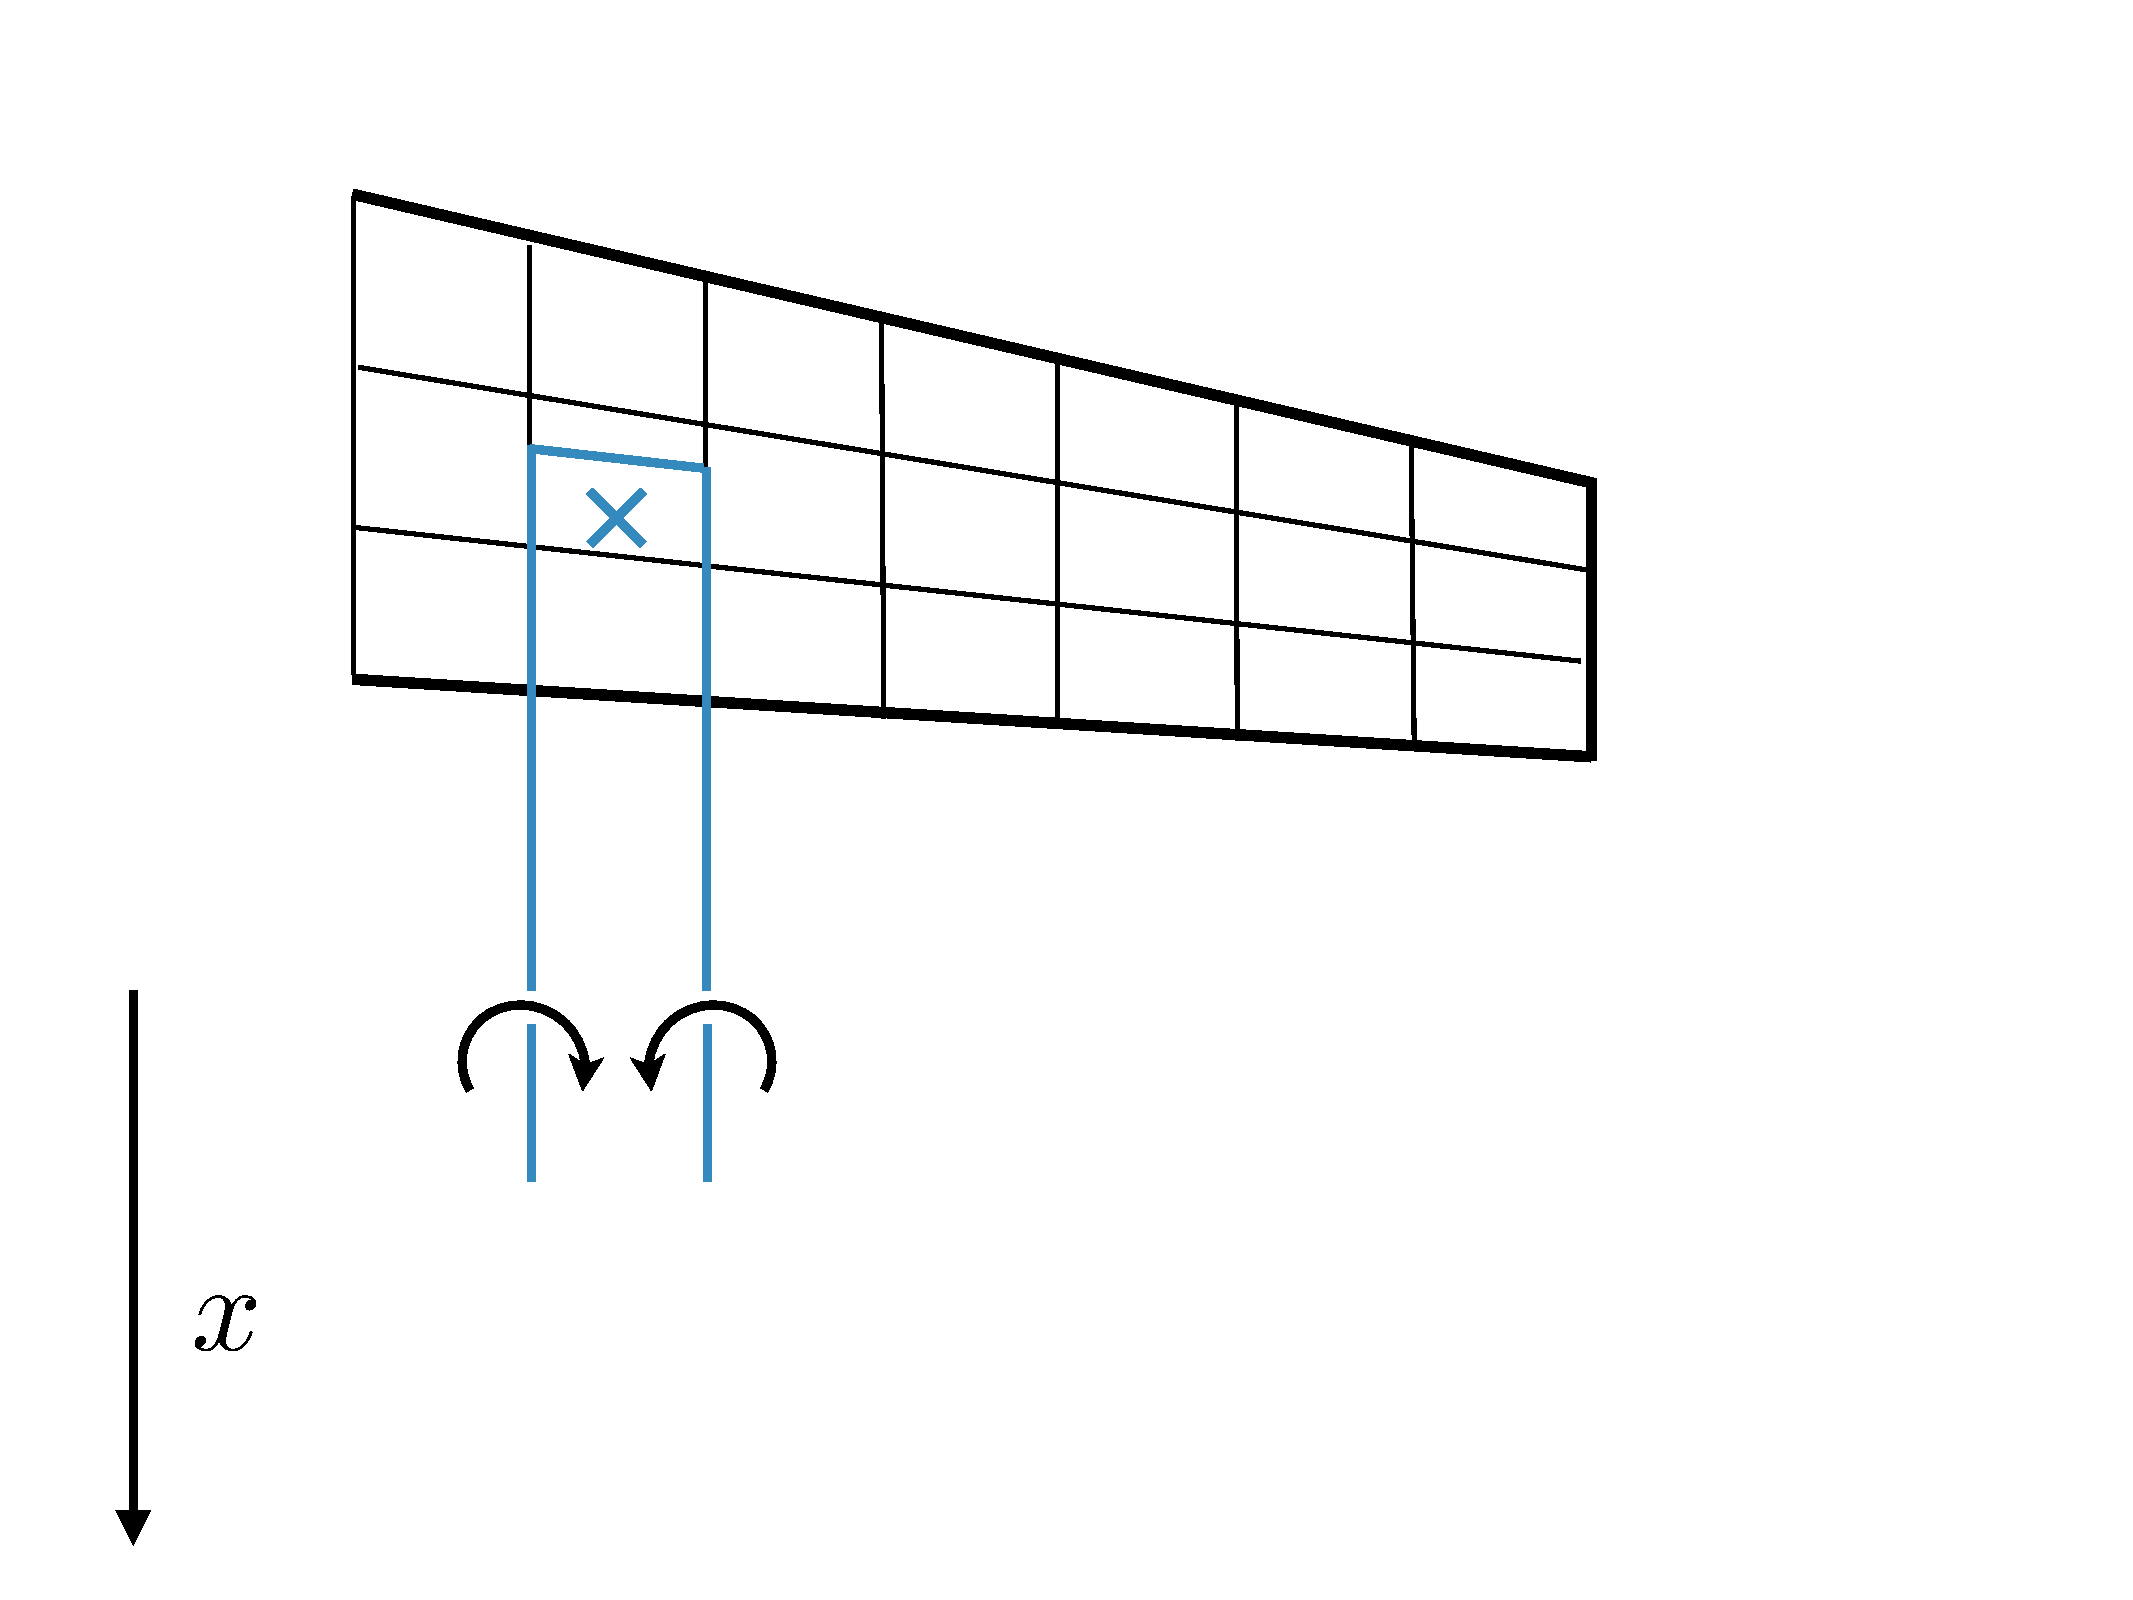
\includegraphics[width=2.5in]{figs/horseshoe}
\caption{An example paneling on a lifting surface. A horseshoe vortex is depicted on one panel, and each panel will have its own horseshoe vortex.  The x denotes the control point for the given panel.}
\label{fig:horseshoe}
\end{figure}

A VLM use the thin airfoil assumption so that  lifting surfaces are flat (not curved).  W wing may be represented with multiple flat surfaces, for example a wing and winglets.  Curved surfaces require a more general 3D panel method.

Although in general a VLM can have both spanwise and chordwise panels, in our case we only use one chordwise panel.  This modeling choice is called a Weissinger formulation [ref], and is appropriate for high aspect ratio wings where resolving the chordwise pressure distribution is of less interest.  


% \section{Boundary Conditions}

Because the vortex filaments automatically satisfy the governing equations, the only remaining conditions to satisfy are flow tangency and the Kutta condition.  Flow tangency means that the normal component of the velocity must be zero at the surface, and this condition we apply at select control points.  Because each horseshoe vortex has a constant (as yet unknown) strength, we can only have one control point per panel, thus maintaining an equal number of unknowns and equations.  The control point was denoted as an x in \cref{fig:horseshoe}, although its proper location is not yet determined.



% The coordinate system aligns the $+x$ axis with the freestream, the $+z$ axis is vertical and the $+y$ axis out the right wing.  Aligning with the $+x$ axis makes it simpler to impose a drag-free wake, as will be discussed.  The downside is that this choice of coordinate system means that an aircraft at an angle of attack or sideslip would need to be rotated.  However, consistent with thin airfoil theory, we do not rotate the geometry (for angle of attack, sideslip, or twist), but rather impose the rotation in the boundary condition.  This approximation is very slight as long as the angles are not large.  Large angles would not be physically consistent anyway with this formulation because viscous effects would be important and irrotational flow requires an inviscid assumption.  Dihedral, on the other hand, is a potentially large angle and that rotation must be reflected in the geometry definition.  The benefit of not rotating the geometry is that the number of coordinate systems is simplified considerably and 

A vortex lattice method uses what is called a lumped vortex method, this means that distributed vorticity along each panel is all lumped into one vortex as shown below.  Even with multiple chordwise panels, this approach is still used, just with the vorticity lumped into separate vortices for each chordwise panel.
\begin{center}
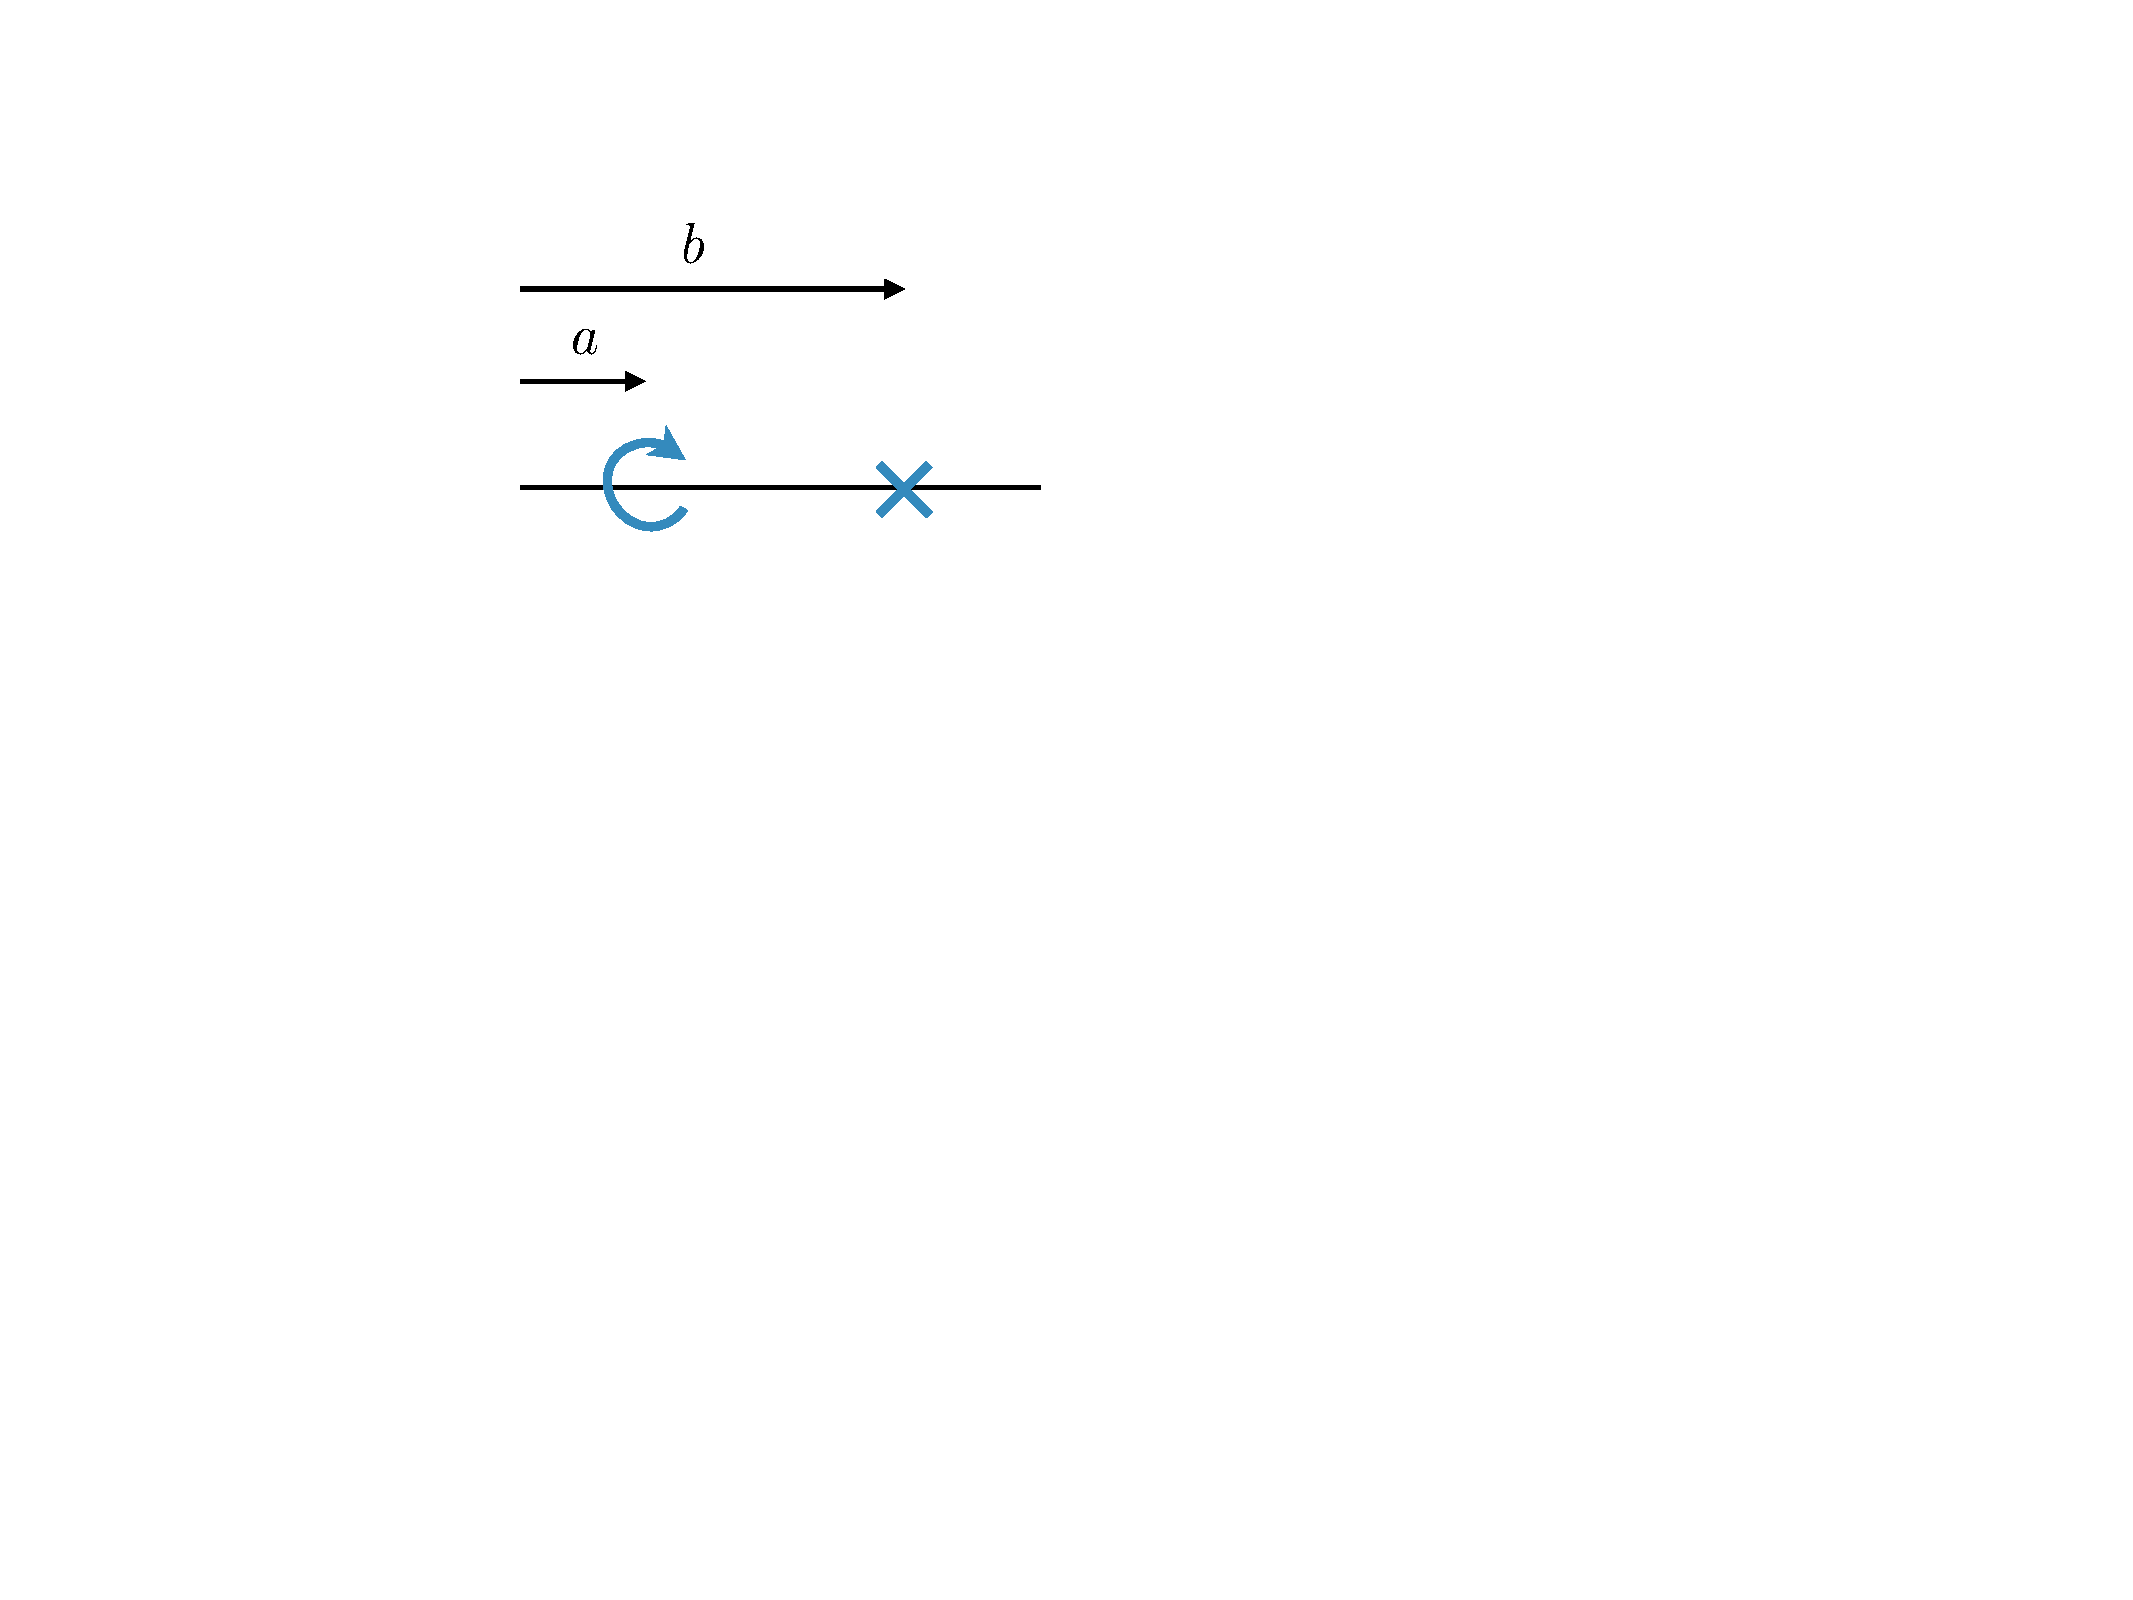
\includegraphics[width=1.5in]{figs/lumped-vortex}
\end{center}
We now have a choice on where to place the lumped vortex, and the control point.  The typical approach can be motivated by assuming that the airfoil has parabolic camber of a generic form.  Because we have only one chordwise control point we cannot resolving flow tangency at multiple points along the camber line, and so it makes sense to impose the camber in the placement of the control point.  A parabolic camber is a reasonable approximation for a general camber line.  This means that the camber line is described by:
\begin{equation}
\bar{y} = 4 \epsilon \frac{x}{c} (c - x)
\end{equation}
Note that at $x = 0$ or $x = c$ the camber goes to zero as expected.  At the midpoint the camber normalized by chord is $\epsilon$, thus $\epsilon$ is a free parameter that governs the maximum amount of camber.  If we use thin-airfoil theory it is straightforward to show that the lift per unit span produced by this camber line is:
\begin{equation}
L^\prime = \pi \rho V_\infty^2 c (\alpha + 2 \epsilon)
\end{equation}
Using the Kutta-Joukowski theorem, we can solve for the corresponding circulation:
\begin{align}
L^\prime = \rho V_\infty \Gamma &= \pi \rho V_\infty^2 c (\alpha + 2 \epsilon)\\
\Rightarrow \Gamma &= \pi V_\infty c (\alpha + 2 \epsilon)
\end{align}
The boundary condition we need to satisfy is flow tangency at the control point.  Using the normal thin-airfoil-theory boundary condition for the camber portion:
\begin{equation}
v_c = V_\infty \left(\frac{d\bar{y}}{dx} - \alpha \right)
\end{equation}
where $v_c$ is the velocity induced by the vorticity distribution, which in this case is a lumped point vortex:
\begin{equation}
-\frac{\Gamma}{2 \pi (b - a)} = V_\infty \left(\frac{d\bar{y}}{dx} - \alpha \right)
\end{equation}
We now insert the slope of the camber line, still using the parabolic camber, evaluated at the control point $x = b$:
\begin{equation}
-\frac{\Gamma}{2 \pi (b - a)} = V_\infty \left(4 \epsilon \left(1 - 2 \frac{b}{c} \right) - \alpha \right)
\end{equation}
We now substitute the circulation we found for the parabolic camber into the above expression, which after some rearranging results in:
\begin{equation}
{\color{blue}\frac{c}{b - a}} \alpha + {\color{red}\frac{2c}{b -1}} \epsilon = {\color{blue}2} \alpha - {\color{red}8\left(1 - 2 \frac{b}{c} \right)}\epsilon
\end{equation}
If we want this boundary condition to be satisfied for any angle of attack, and any amount of camber, then we need to equate the two blue terms, and equate the two red terms separately.  This leads to two equations for two unknowns with the solution:
\begin{align}
a &= \frac{1}{4} c\\
b &= \frac{3}{4} c
\end{align}
In other words, the lumped vortex should be placed at the section quarter-chord, and the control point at three quarters-chord.  The placing of the vortex at the quarter chord could also be motivated by the fact that it is the location of the aerodynamic center according to thin airfoil theory.  Note that this result does not depend on the value of $\epsilon$ and thus is independent of the amount of camber (even zero camber), with the assumptions of parabolic camber and thin airfoil theory.  Also note that in using the lift result from thin airfoil theory we have implicitly imposed the Kutta condition already. Thus, with only one chordwise panel, we only need to satisfy flow tangency at the control points.

% A similar approach can be used for multiple chord-wise panels, where the bound vortex is placed at the quarter chord of each panel, and the control point at three quarters-chord of each panel.  

It is generally convenient in a vortex lattice method (VLM) to separate the geometry-dependent terms from the circulation (strength of each horseshoe vortex).  These geometry dependent terms will be called influence coefficients in the following sections.

\section{Aerodynamic Influence Coefficients (AIC)}


% There are two natural choices for coordinate systems, each with some minor drawbacks.  We will choose a third that is somewhat approximate, but consistent with the assumptions already used in a VLM and greatly simplifies the problem specification.  The first choice is a body-aligned coordinate system.  This allows for straightforward specification of the geometry and velocity vectors.  However, the freestream is in general not aligned with the aircraft.  For reasons we will discuss later we want to use a drag-free wake, which means that the wake should be aligned with the freestream.  Wake vortices that are aligned with the freestream implies that the horseshoe vortices will have a bend in them and the Trefftz plane will require a projection onto a different coordinate system.  Additionally, the calculation of lift requires a rotation.  These are of course not difficult calculations, but do complicate the visualization somewhat.  

% A second choice is to use a wind-aligned coordinate system.  This makes specifying the drag-free wake easy (it just goes straight back in the $+x$ direction), the Trefftz projection requires no calculation, and lift is in the $+z$ direction.  The downside is that the aircraft geometry would need to be rotated for angle of attack and sideslip.  Also, the horseshoe vortices would still be bent.  Both of these require working with multiple coordinate systems and rotating between them.  

% A third option, which is what we use, is to choose a wind-aligned axis (freestream in the $+x$ direction) but not rotate the geometry when creating the vortices.  The rotation is still used in the boundary condition (in other words the boundary condition is still exact).  The choice to not rotate the geometry in defining the horseshose vortices is consistent with how the VLM is modeled.  Wing twist is already modeled only in the boundary condition and horseshoe vortices are not rotated with the local twist angle.  If horseshose vortices were rotated on each section we could have numerical issues with nonaligned, but nearby vortices.  For a planar wing, angle of attack could be complete encapsulated in the twist variable (though not for a nonplanar wing) so it makes sense to treat these consistently.  The only approximation then in this formulation is that we are not using a bent horseshoe vortex.  This could be considered a small angle assumption for angle of attack, sideslip, and twist and only small angles are physically meaningful anyway since the flow is irrotational and hence inviscid.  Dihedral, on the other is a (potentially) large angle and so the vortices must  and so we Additionally, the drag-free wake is a nonphysical representation of the wake to begin with so it is difficult to argue that a bent horseshoe vortex is more preferably then a straight horseshoe vortex.  This modeling choice then has essentially no real drawback and considerably simplifies our representation as we only need one coordinate system.  


As noted the control point on each panel is at the section's three quarters-chord point.  There is one control point for each panel.  The boundary condition is flow tangency:
\begin{equation}
    \vec{V}_n|_{cp} = 0
\end{equation}
where the $cp$ subscript denotes a control point, and the boundary condition is applied at each control point separately.  The velocity can be broken up into four terms: the freestream velocity, velocity from rigid-body rotation, self-induced velocity from the vortices, and other external velocity sources such as upstream wakes or gusts.  The freestream velocity is defined as the negative of the translational motion of the vehicle (thus it is constant for the entire aircraft, unlike gusts which may vary along the aircraft and are lumped in $\vec V_{other}$). The flow tangency boundary condition is thus:
\begin{equation}
    \left[(\vec{V}_\infty - \vec{\Omega} \times \vec{r}_b + \vec{V}_{ind} + \vec{V}_{other}) \cdot \hat{n} \right]_{cp}= 0
\end{equation}
where $\vec{r}_b$ is a vector from the aircraft center of gravity to a point of interest.  We will move the induced term to one side, and all other terms to the other side (where the cp subscript is dropped for simplicity in notation):
\begin{equation}
    \vec{V}_{ind} \cdot \hat{n} = - (\vec{V}_\infty - \vec{\Omega} \times \vec{r} +  \vec{V}_{other}) \cdot \hat{n}
\end{equation}
To keep the notation simple we will denote the velocity on the right-hand side as $\vec V_{ext}$.
\begin{equation}
\vec{V}_{ind} \cdot \hat{n} = - \vec{V}_{ext} \cdot \hat{n}
\end{equation}
% Each normalwash is a scalar and thus independent of the coordinate system.  In other words, we can use different coordinate systems to compute different portions of the sum, as long as the coordinate system is consistent for the two vectors in the dot product.  All of the external velocity computations  will use body axes, and the induced velocities will use wind axes.  In other words:
% \begin{equation}
% \vec{V}_{ind, w} \cdot \hat{n}_w = - \vec{V}_{ext, b} \cdot \hat{n}_b
% \label{eq:flowtangency}
% \end{equation}
In general the rotational velocity, self-induced velocity, and external velocity all vary along the aircraft, and so this boundary condition will be applied at each control point $i$.
\begin{equation}
\vec{V}_{ind, i} \cdot \hat{n}_i = - \vec{V}_{ext, i} \cdot \hat{n}_i
\label{eq:flowtangency}
\end{equation}

\subsection{External Velocities}

Angle of attack and sideslip angle are defined in the standard way (\cref{fig:alphabeta2}).  In this case, the the freestream velocity vector in the body axes is: 
\begin{equation}
    \vec{V}_{\infty} = V_\infty
    \begin{bmatrix}
    \cos\alpha\cos\beta\\
    -\sin\beta\\
    \sin\alpha\cos\beta
    \end{bmatrix}
    \label{eq:Vinf}
\end{equation}
% Note that the subscript distinguishes that this is the velocity in the body axes, not in the wind axes that we will be using in other parts of the problem $V_{\infty,w} = V_\infty \hat{x}_w$.

\begin{figure}[htbp]
\centering
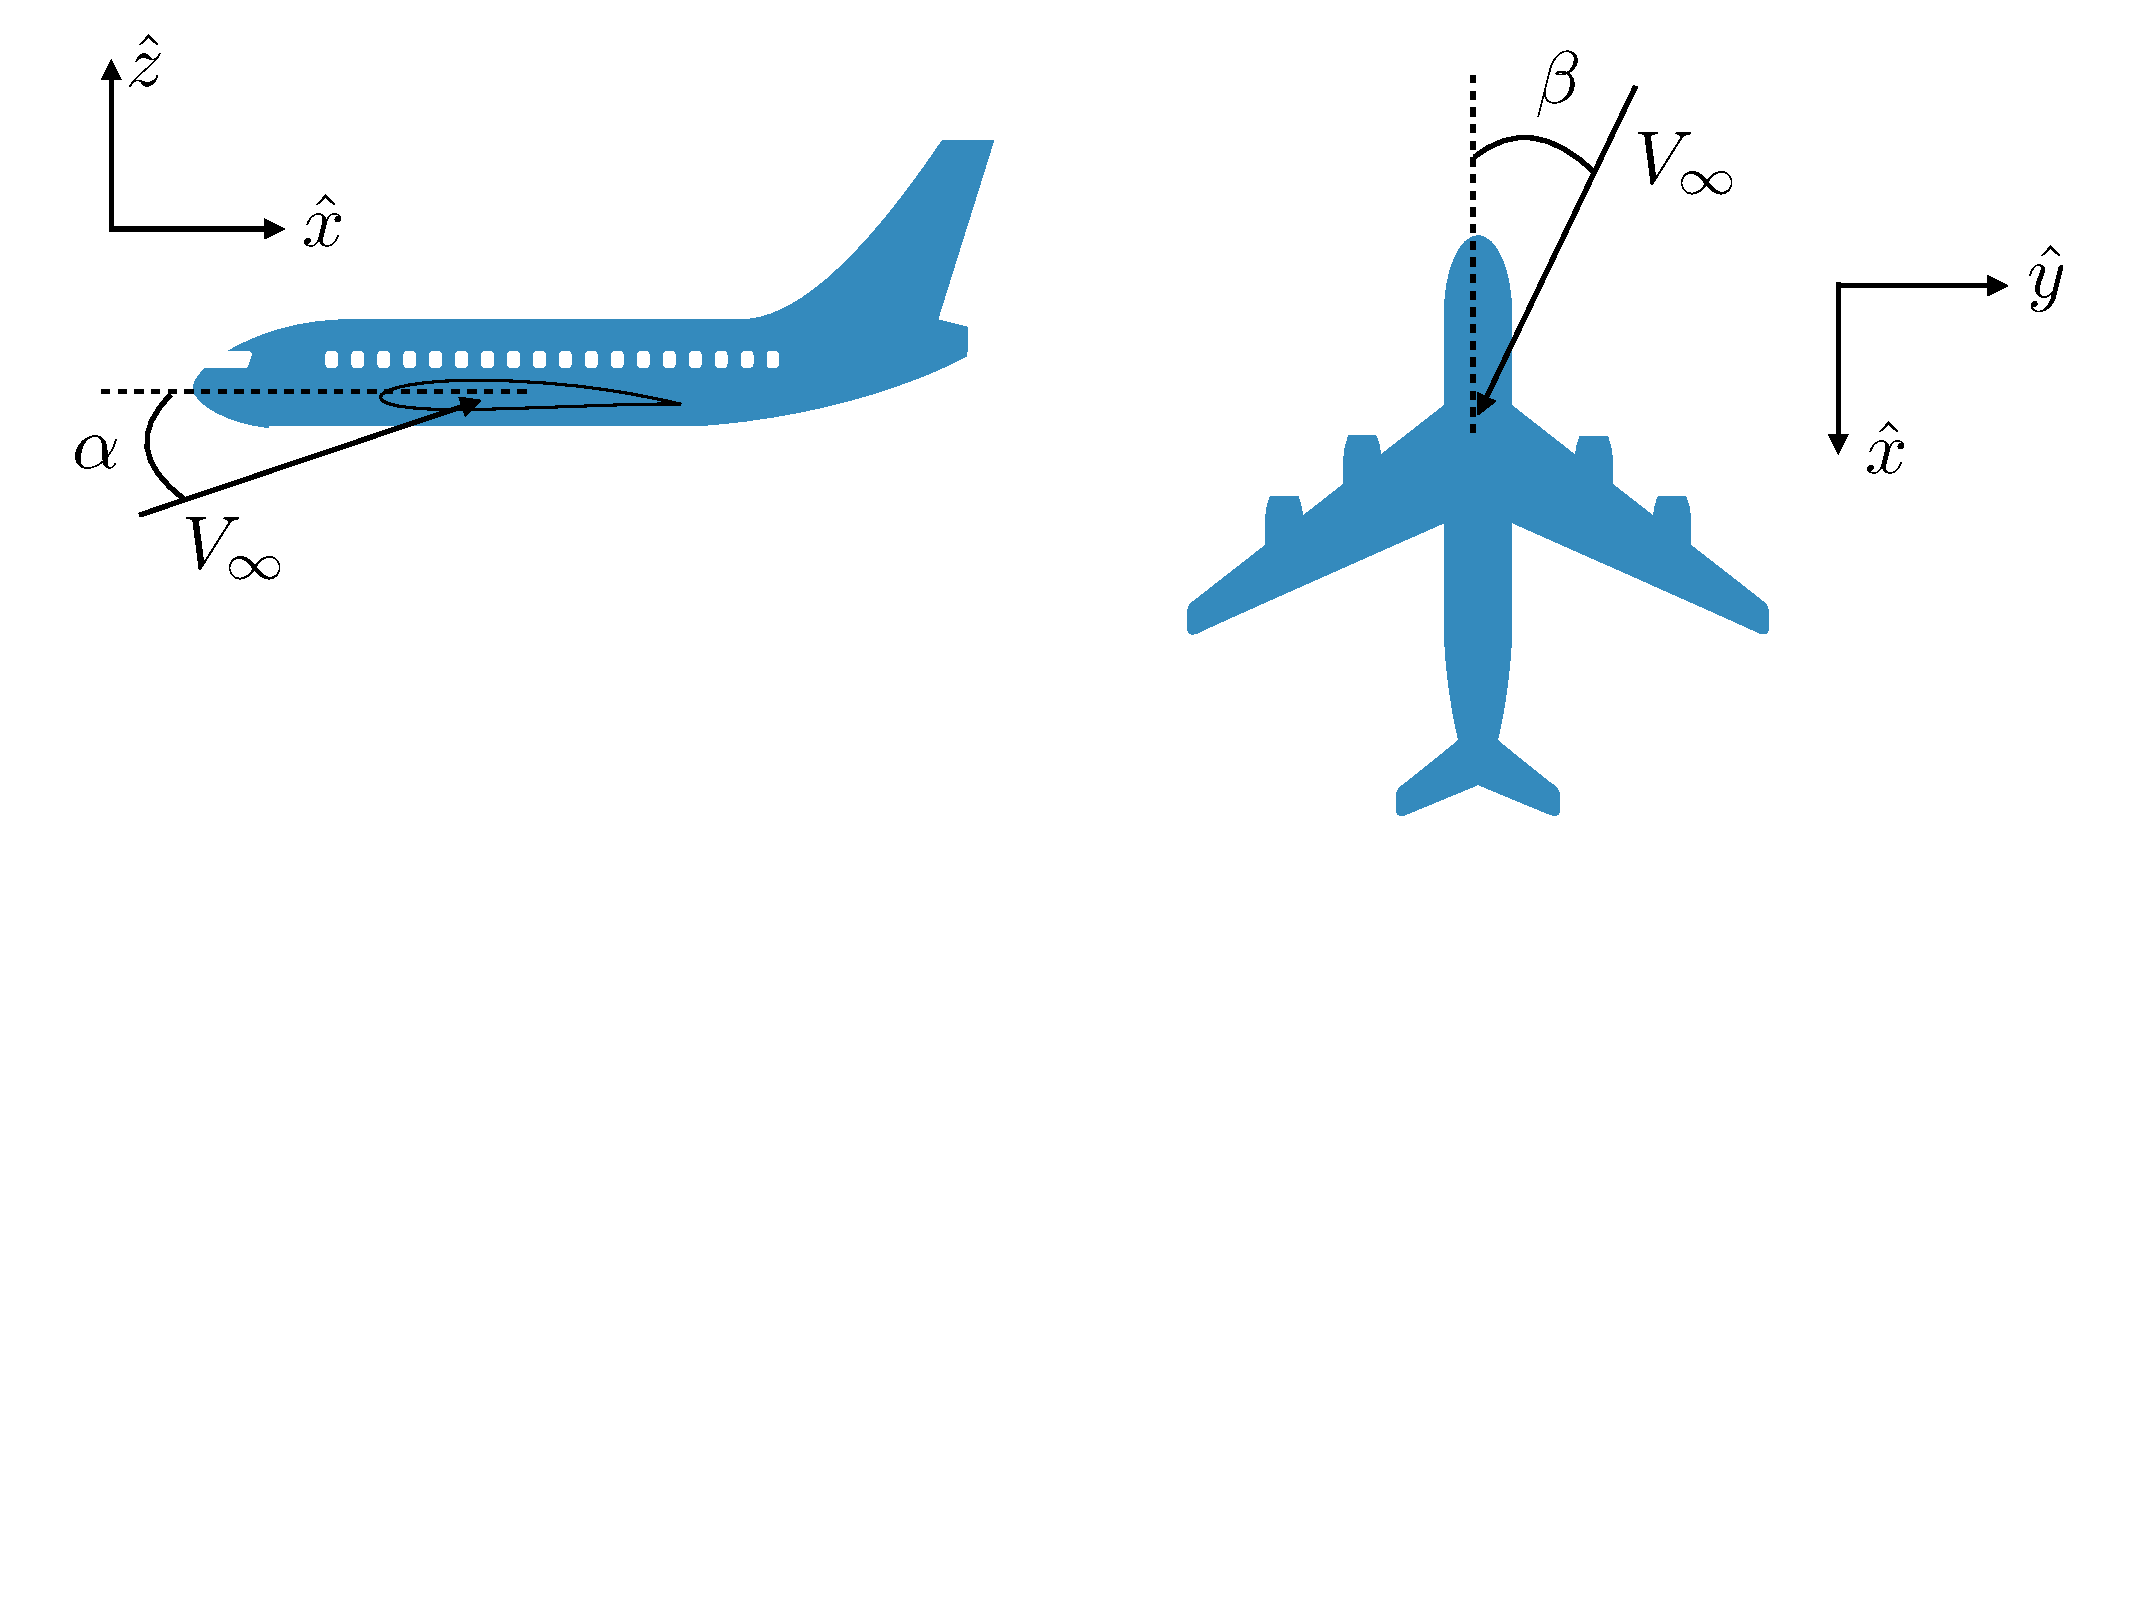
\includegraphics[width=4.0in]{figs/alphabeta2}
\caption{Angle of attack and sideslip shown in body axes.}
\label{fig:alphabeta2}
\end{figure}

% Using a different definition for the freestream velocity appears to be inconsistent with our choice to define $V_\infty$ in the $+x$ direction, but it actually is not.  To see this more rigorously.  Let's consider the case where we keep the velocity vector in the $+x$ direction, but do rotate the geometry.  In that case, the angle of attack and sideslip would need to be accounted for in $\hat{n}$ which defines the normal vector to each panel in our wind axes.  The transformation matrix from body axes to wind axes (using the standard aerodynamic coordinate system we have been using, and not a standard dynamics coordinate system) is:
% \begin{equation}
% \hat{n}_w = 
% \begin{bmatrix}
% \cos\beta & -\sin\beta & 0 \\
% \sin\beta & \cos\beta & 0 \\
% 0 & 0 & 1\\
% \end{bmatrix}
% \begin{bmatrix}
% \cos\alpha & 0 & \sin\alpha \\
% 0 & 1 & 0\\
% -\sin\alpha & 0 & \cos\alpha \\
% \end{bmatrix}
% \hat{n}_b
% \end{equation}
% Thus, 
% \begin{align}
% \vec{V}_\infty \cdot \hat{n}_w &= \vec{V}_\infty \cdot R_\beta R_\alpha \hat{n}_b\\
% &= V_\infty \hat{x} \cdot R_\beta R_\alpha \hat{n}_b\\
% \end{align}


The rotational velocity is defined about the center of gravity and is simply:
\begin{equation}
    \Omega =
    \begin{bmatrix}
    \Omega_x\\ \Omega_y\\ \Omega_z
    \end{bmatrix}
\end{equation}
The radial vector used in determining rotational velocities is the distance from the aircraft center of gravity to the control point of interest:
\begin{equation}
\vec{r}_i = \vec r_{cp, i} - \vec r_{cg}
\end{equation}
Because we only have one chordwise panel, it doesn't make sense to use camber in defining the normal direction (and camber was implicitly accounted for in the use of positioning the bound vortex and control point).  The normal vector is a function of the local twist and dihedral as shown in the figure below.  Twist cannot be lumped with angle of attack for nonplanar wings.  Imagine the twist on a winglet (sometimes called the cant angle), it moves  the surface in a very different way than changing the angle of attack of the entire aircraft.
\begin{center}
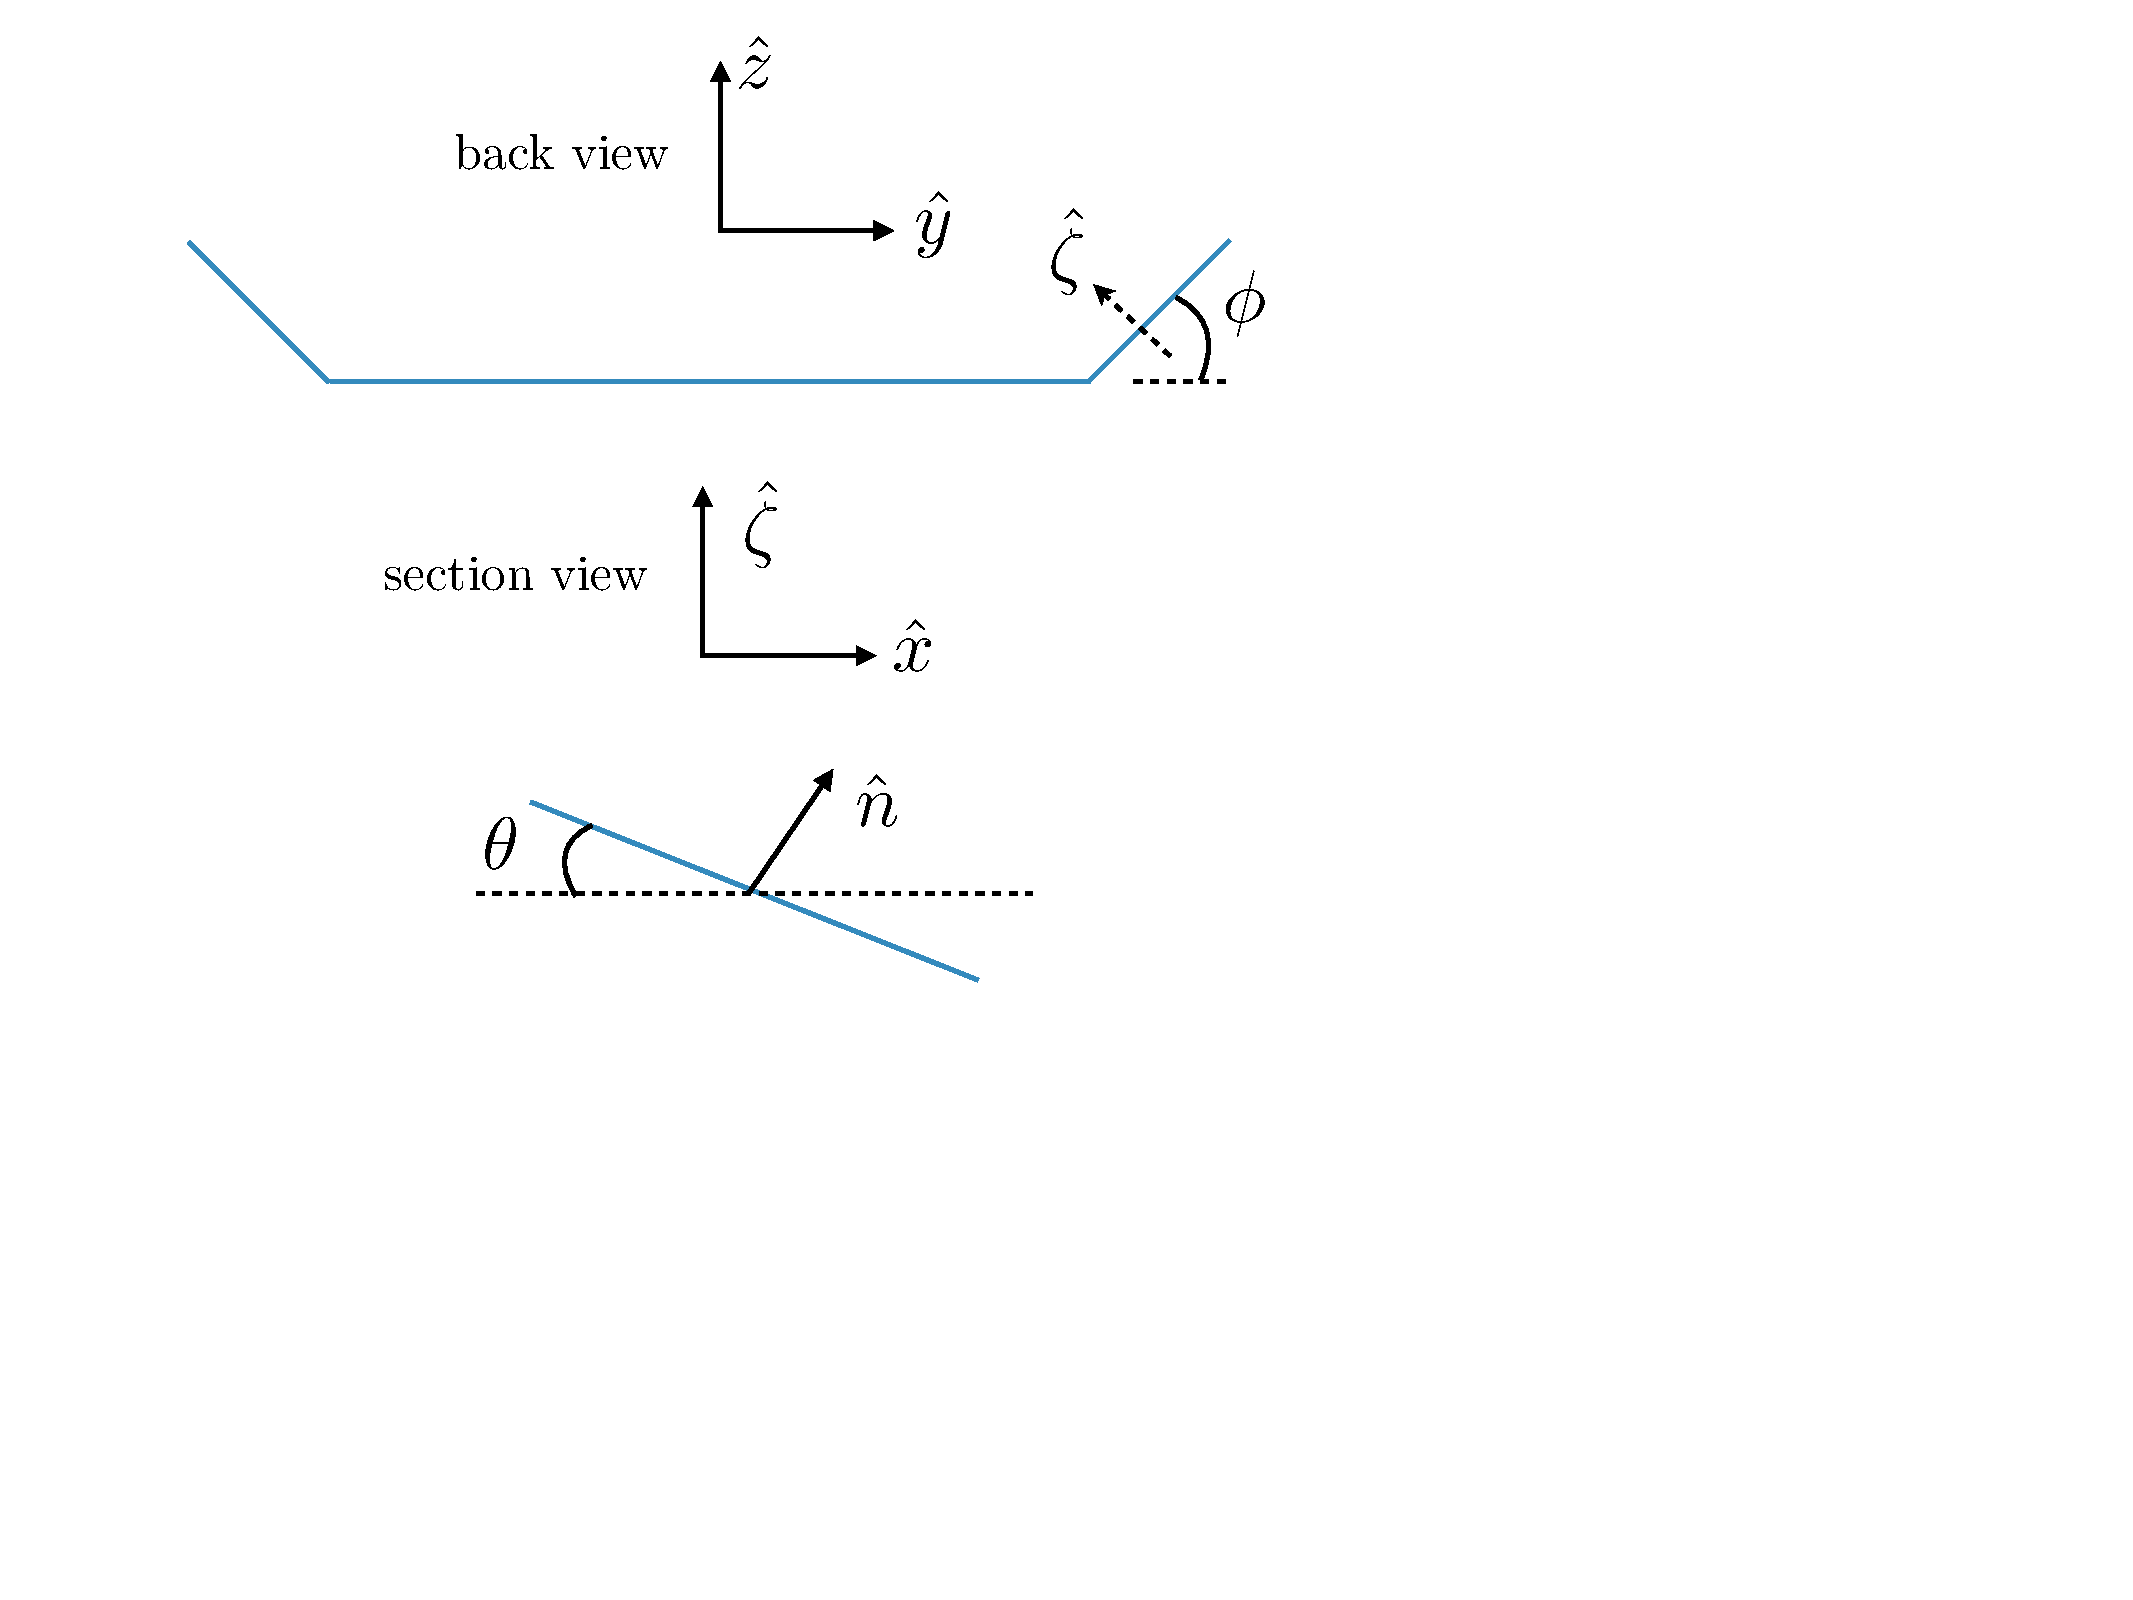
\includegraphics[width=2.5in]{figs/normalvector}
\end{center}
From the figure we can resolve $\hat\zeta$ and $\hat{n}$ into components as follows:
\begin{equation}
\hat\zeta = -\sin\phi \hat{y} + \cos\phi \hat{z}
\label{eq:hatzeta}
\end{equation}
\begin{align}
\hat{n} = \sin\theta \hat{x} + \cos\theta \hat{\zeta}
\label{eq:hatn}
\end{align}
Substituting \cref{eq:hatzeta} into \cref{eq:hatn} yields:
\begin{equation}
    \hat{n} =
    \begin{bmatrix}
        \sin\theta\\
        -\cos\theta\sin\phi\\
        \cos\theta\cos\phi\\
    \end{bmatrix}
\end{equation}
Using the panel discretization
\begin{align}
    \sin\phi_i &= \frac{z_{i+1} - z_i}{\sqrt{(y_{i+1} - y_i)^2 + (z_{i+1} - z_i)^2}}\\
    \cos\phi_i &= \frac{y_{i+1} - y_i}{\sqrt{(y_{i+1} - y_i)^2 + (z_{i+1} - z_i)^2}}
\end{align}
% Other induced velocities will just be defined as a user-supplied vector at each control point.

\subsection{Induced Velocities}

% A wind-aligned coordinate system is easiest in computing the induced velocities as it allows for the trailing vortices to be in the $+x$ direction.  This means we need to convert our normal vector from the body axes to the wind axes, which is done through the two rotation matrices as shown below.
% \begin{equation}
% \hat{n}_w = 
% \begin{bmatrix}
% \cos\beta & -\sin\beta & 0 \\
% \sin\beta & \cos\beta & 0 \\
% 0 & 0 & 1\\
% \end{bmatrix}
% \begin{bmatrix}
% \cos\alpha & 0 & \sin\alpha \\
% 0 & 1 & 0\\
% -\sin\alpha & 0 & \cos\alpha \\
% \end{bmatrix}
% \hat{n}_b
% \end{equation}

% However, this presents a modeling choice.  Vortices could go straight back in $+x$ from the quarter chord or could follow along the wing surface to the trailing edge and then go straight back in $+x$ [fig].  We will choose the former, as this is consistent with thin airfoil theory which VLM is based on.  Wing twist is already modeled only in the boundary condition---horseshoe vortices are not rotated with the local twist angle.  Doing so would create numerical issues with nonaligned, but nearby vortices.  For a planar wing, angle of attack could be complete encapsulated in the twist variable (though not for a nonplanar wing) so it makes sense to treat these consistently. Essentially this is a small angle approximation for angle of attack, sideslip, and twist.  Realistically, only small angles are physically meaningful for these quantities anyway otherwise viscous effects would be important and flow would not be irrotational.  Dihedral, on the other is a (potentially) large angle and so the vortices must follow wing dihedral. Angle of attack, sideslip, and twist are still accounted for in the boundary conditions.

From the Biot-Savart law the induced velocity from a vortex filament is given by the integral
\begin{equation}
    \vec{V}_{ind-one} = \frac{\Gamma}{4\pi}\int \frac{dl^\prime \times (r - r^\prime)}{|r - r^\prime|^3}
\end{equation}
then the induced velocity from all of the vortex filaments at control point $i$ is
\begin{equation}
    \vec{V}_{ind, i} = \sum_j \frac{\Gamma_j}{4\pi}\int_j \frac{dl_j \times (r_i - r_j)}{|r_i - r_j|^3}
\end{equation}
which we can reexpress as
\begin{equation}
    \vec{V}_{ind, i} = \sum_j \hat{V}_{ij} \Gamma_j
\end{equation}
where $\hat{V}$ is the induced velocity at the control point, for unit circulation.  Thus, the boundary condition at the $i$th control point (\cref{eq:flowtangency}) becomes:
\begin{equation}
\sum_j \Gamma_j \hat{V}_{ij} \cdot \hat{n}_{i} = - \vec V_{ext,i} \cdot \hat{n}_{i}
\end{equation}
Each control point is one equation, and putting them all together forms a linear system of equations:
\begin{equation}
[AIC] \Gamma = b 
\label{eq:linearsystem}
\end{equation}
where 
\begin{equation}
b_i = - \vec V_{ext, i} \cdot \hat{n}_{i}
\label{eq:rhs}
\end{equation}
and the aerodynamic influence coefficient matrix is given by:
\begin{equation}
AIC_{ij} = \hat{V}_{ij} \cdot \hat{n}_{i}
\end{equation}
The main challenge then is to determine $\hat{V}_{ij}$


From the Biot-Savart law the induced velocity of a vortex filament is:
\begin{equation}
\vec{V} = \frac{\Gamma}{4 \pi} \int \frac{d \vec{l} \times \vec{r}}{|\vec{r}|^3}
\label{eq:biotsavart}
\end{equation}
\begin{figure}[htbp]
\centering
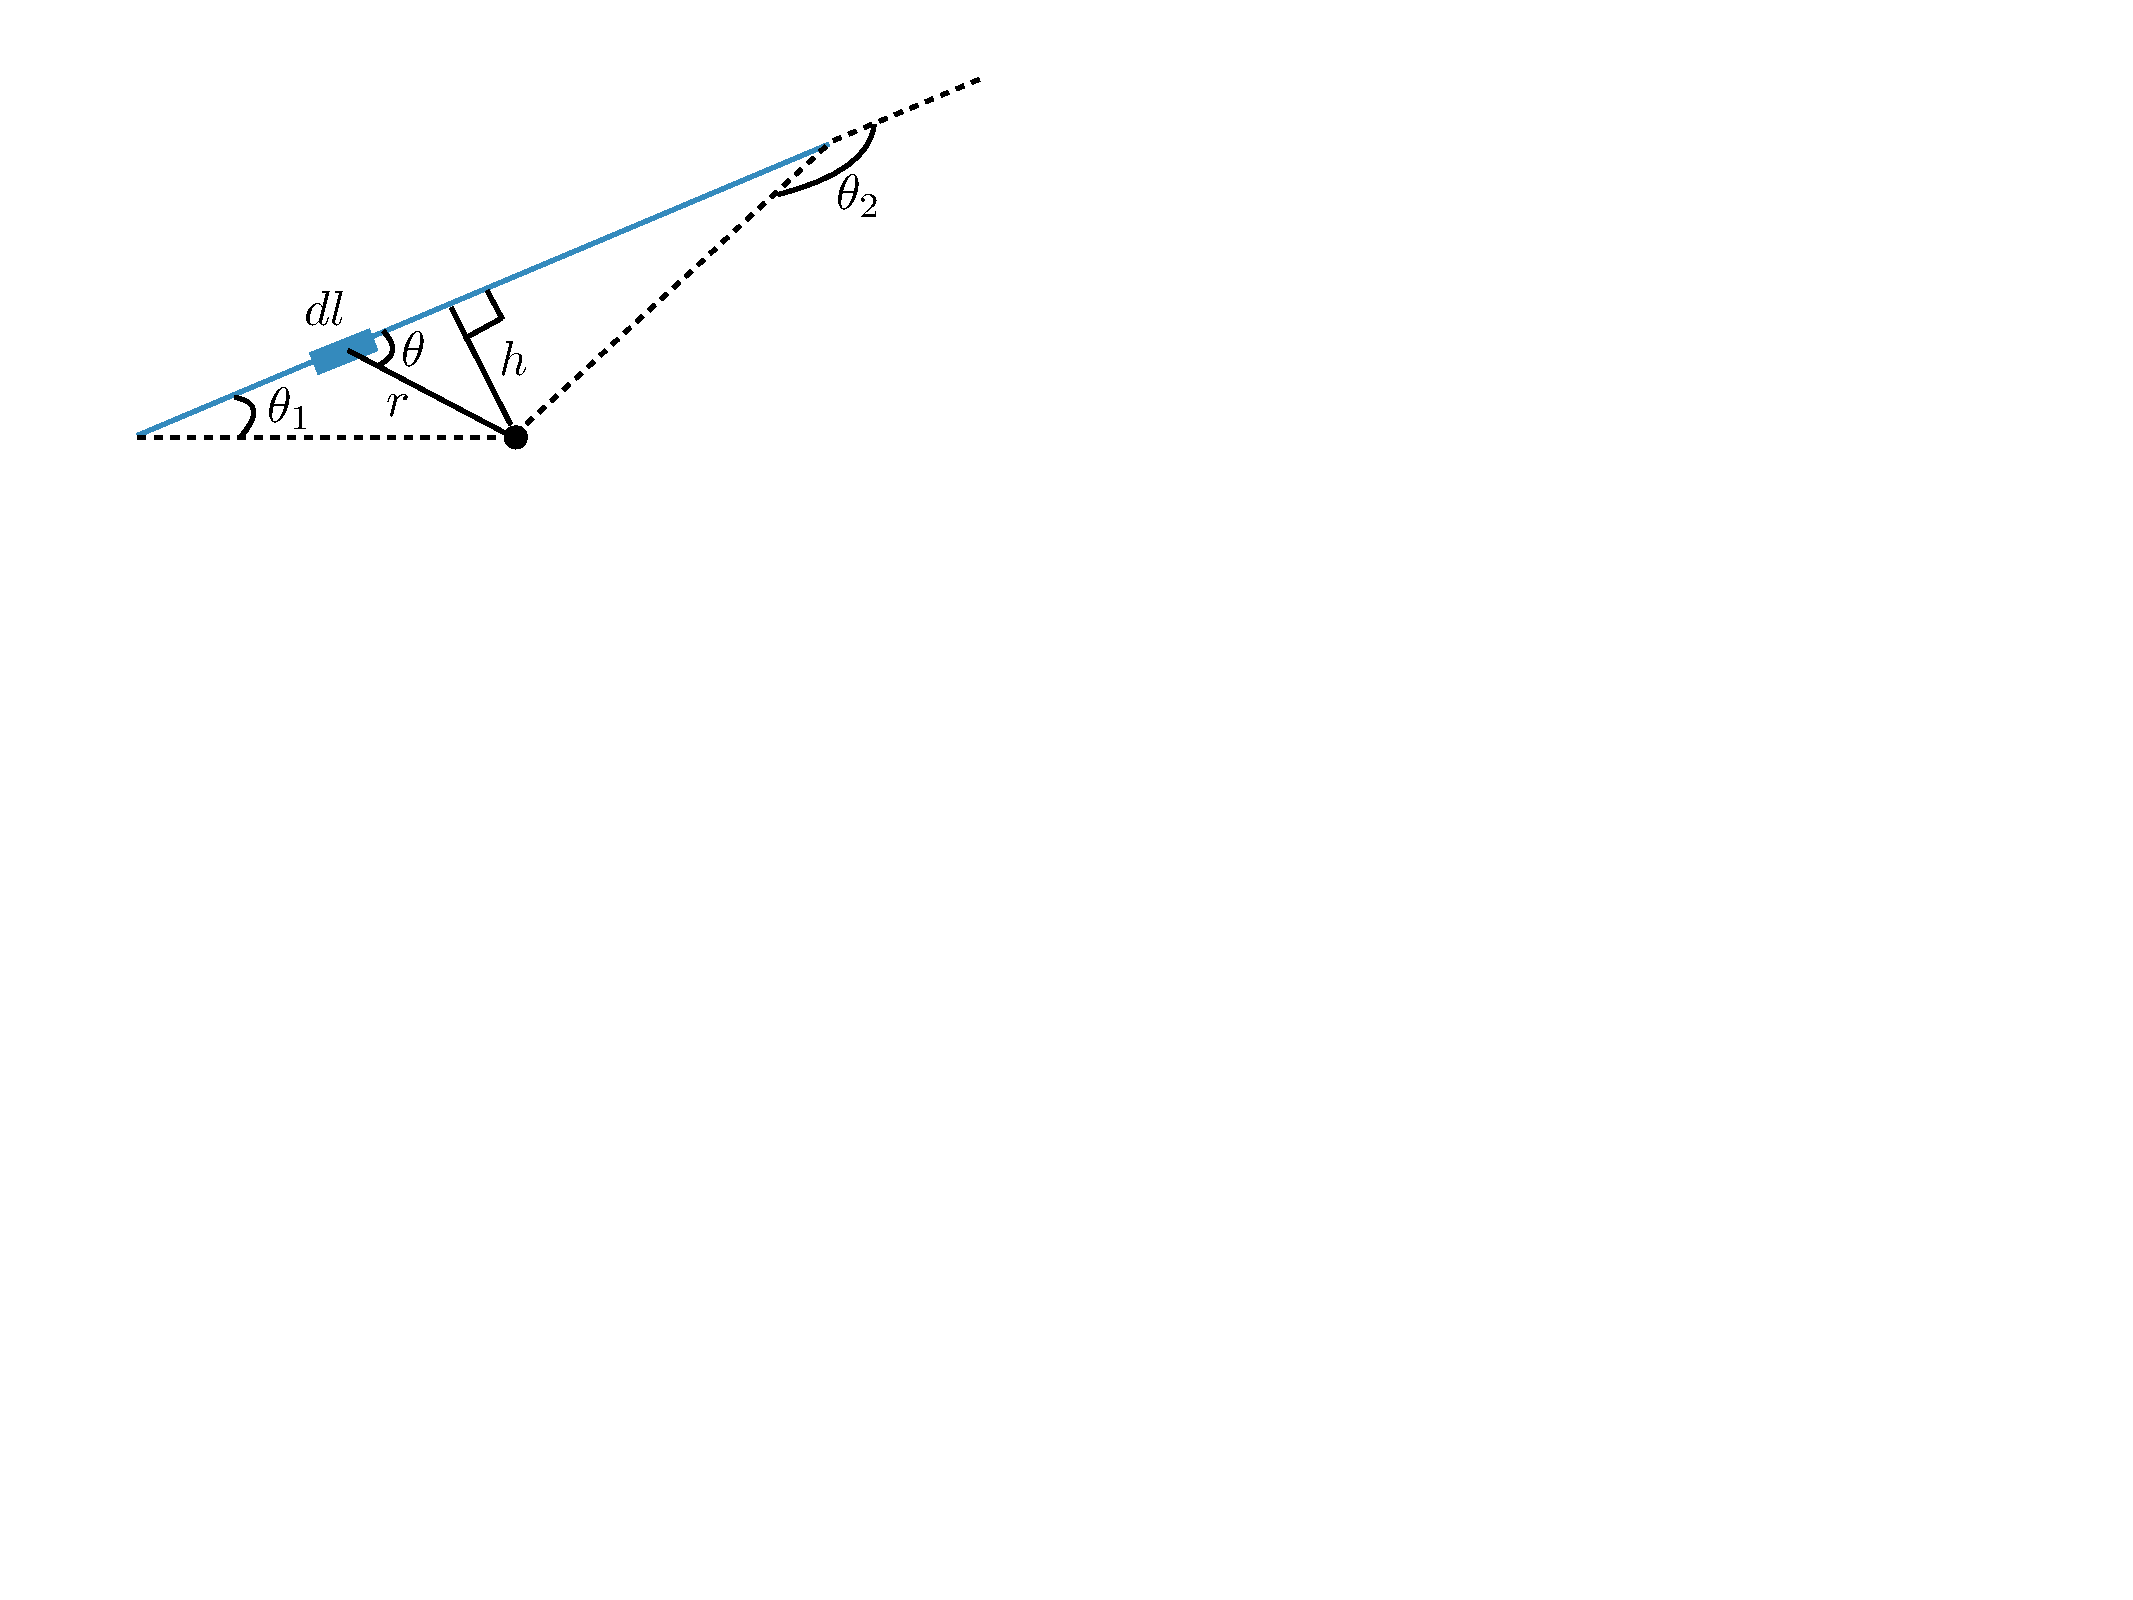
\includegraphics[width=2.5in]{figs/filament}
\caption{caption}
\label{fig:filament}
\end{figure}
Consider the vortex filament shown in \cref{fig:filament}.  The segment $d\vec{l}$ is a distance $r$ away from a point we want to evaluate the induced velocity at.  The distance $h$ is the perpendicular distance from the vortex to the point.  For the moment we won't worry about directions, for a filament it is obvious from the geometry, but later we will be more rigorous about directions.  
The magnitude of the cross product is:
\begin{equation}
d\vec{l} \times \vec{r} = dl r \sin\theta
\end{equation}
From the geometry we see that 
\begin{align}
\sin\theta &= \frac{h}{r}\\
\tan\theta &= \frac{h}{l_h - l}
\end{align}
where $l_h$ is the point on the vortex filament that intersects with $h$ (a constant value), and $l$ is a variable that moves along the filament.  We use the first expression to solve for $r$ and the second to solve for $dl$:
\begin{align}
r &= \frac{h}{\sin\theta}\\
dl &= \frac{h}{\sin^2\theta} d\theta
\end{align}
Making these substitutions into \cref{eq:biotsavart} yields:
\begin{equation}
|\vec{V}| = \frac{\Gamma}{4 \pi} \int_{\theta_1}^{\theta_2} \frac{\sin\theta}{h} d\theta
\end{equation}
The distance $h$ is a constant so it can be pulled out of the integral leaving us with a simple answer for the magnitude of the induced velocity from the vortex segment:
\begin{equation}
V_\theta = \frac{\Gamma}{4 \pi h}(\cos\theta_1 - \cos\theta_2)
\end{equation}

We will now use this expression for a horseshoe vortex, which is comprised of three segments.  This time we will need to be more careful with directions.  First, we convert this expression in terms of vectors so that we can use it more generally in a computational implementation.  Second, the angles $\theta$ are less convenient to work with, we would prefer to use vectors instead.  We define the quantities $\vec{r}_0$, $\vec{r}_1$ and $\vec{r}_2$ as shown in \cref{fig:vectordef}.  Vector $\vec{r}_0$ starts at one of the vortex filament and ends at the other pointing in the direction of positive circulation according to the right hand rule.  Vector $\vec{r}_1$ points from the start of the filament to the point of interest, and vector $\vec{r}_2$ points from the end of the filament to the point of interest.

\begin{figure}[htbp]
\centering
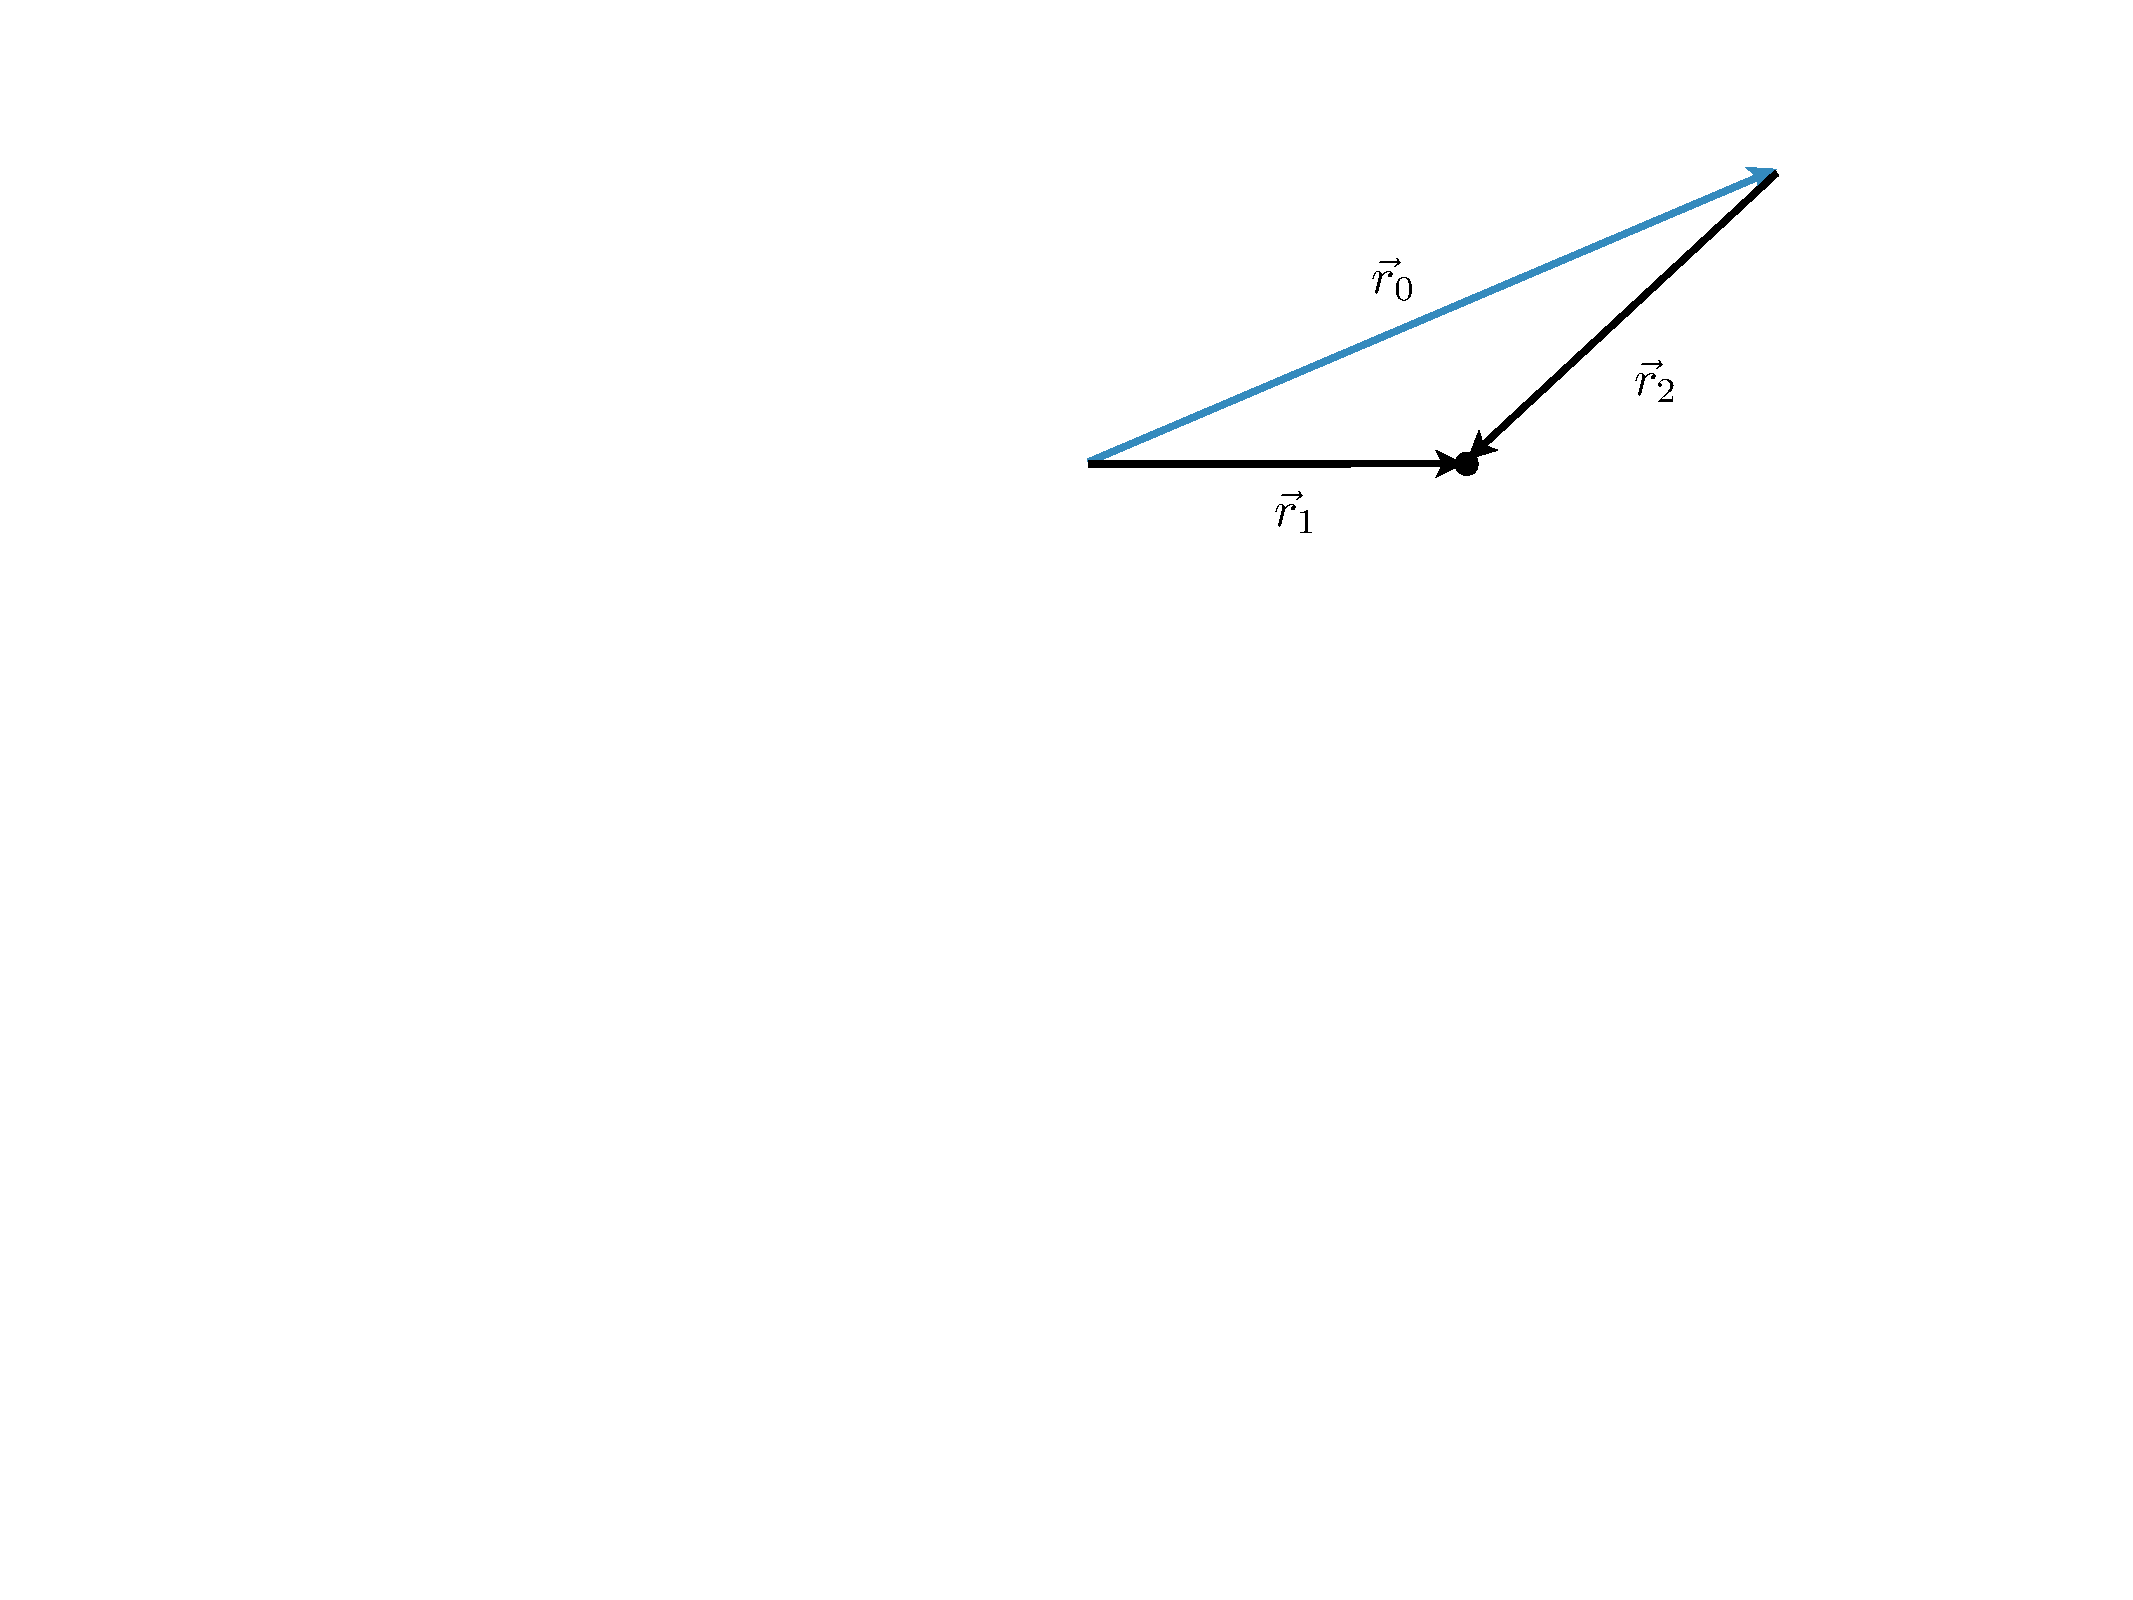
\includegraphics[width=2in]{figs/vectordef}
\caption{}
\label{fig:vectordef}
\end{figure}

We use the definition of the dot product to obtain the angles.
\begin{equation}
\vec{r}_0 \cdot \vec{r}_1 = |\vec{r}_0||\vec{r}_1| \cos\theta_1 \Rightarrow \cos\theta_1 = \frac{\vec{r}_0 \cdot \vec{r}_1}{|\vec{r}_0||\vec{r}_1|}
\end{equation}
\begin{equation}
\vec{r}_0 \cdot \vec{r}_2 = |\vec{r}_0||\vec{r}_2|  \cos\theta_2
\Rightarrow \cos\theta_2 = \frac{\vec{r}_0 \cdot \vec{r}_2}{|\vec{r}_0||\vec{r}_2|}
\end{equation}
The distance $h$ is just $r_1 \sin\theta_1$, but again we want to eliminate the explicit dependence on angles.  Using the definition of the cross product:
\begin{equation}
|\vec{r}_0 \times \vec{r}_1 | = |\vec{r}_0| |\vec{r}_1| \sin\theta_1 
\end{equation}
Thus,
\begin{equation}
h = |\vec{r}_1| \frac{|\vec{r}_0 \times \vec{r}_1 |}{|\vec{r}_0| |\vec{r}_1|} = \frac{|\vec{r}_0 \times \vec{r}_1 |}{|\vec{r}_0|}
\end{equation}
Finally, we need to determine the direction of $V_\theta$.  We have defined $\vec{r}_0$ to correspond to the direction of the circulation $\vec\Gamma$.  Thus, the direction is a unit vector in the direction of $\vec{r}_0 \times \vec{r}_1$.  In other words, 
\begin{equation}
\vec{V}_\theta = V_\theta \frac{\vec{r}_0 \times \vec{r}_1}{|\vec{r}_0 \times \vec{r}_1|}
\end{equation}

Putting all of these pieces together yields:
\begin{align}
    \vec{V}_\theta &= \frac{\Gamma |\vec{r}_0|}{4 \pi |\vec{r}_0 \times \vec{r}_1 |} \frac{\vec{r}_0 \times \vec{r}_1}{|\vec{r}_0 \times \vec{r}_1|} \left(\frac{\vec{r}_0 \cdot \vec{r}_1}{|\vec{r}_0||\vec{r}_1|} - \frac{\vec{r}_0 \cdot \vec{r}_2}{|\vec{r}_0||\vec{r}_2|} \right)\\
    &= \frac{\Gamma}{4 \pi} \frac{\vec{r}_0 \times \vec{r}_1}{|\vec{r}_0 \times \vec{r}_1|^2} \left(\frac{\vec{r}_0 \cdot \vec{r}_1}{|\vec{r}_1|} - \frac{\vec{r}_0 \cdot \vec{r}_2}{|\vec{r}_2|} \right)
\end{align}
To simplify further we can express $\vec{r_0}$ in terms of $\vec{r_1}$ and $\vec{r_2}$:
\begin{equation}
    \vec{r}_0 = \vec{r}_1 - \vec{r}_2
\end{equation}
Making this substitution yields:
\begin{align}
    &= \frac{\Gamma}{4 \pi} \frac{\vec{r}_1 \times \vec{r}_2}{|\vec{r}_1 \times \vec{r}_2|^2} \left(\frac{|\vec{r}_1|^2 - \vec{r}_2 \cdot \vec{r}_1}{|\vec{r}_1|} - \frac{\vec{r}_1 \cdot \vec{r}_2 - |\vec{r}_2|^2}{|\vec{r}_2|} \right)
    \label{eq:almostthere}
\end{align}
We can expand the cross product in the denominator:
\begin{align}
|\vec{r}_1 \times \vec{r}_2|^2 &= (\vec{r}_1 \times \vec{r}_2) \cdot (\vec{r}_1 \times \vec{r}_2)\\
&= (\vec{r}_1 \cdot \vec{r}_1)(\vec{r}_2 \cdot \vec{r}_2) - (\vec{r}_2 \cdot \vec{r}_1)(\vec{r}_1 \cdot \vec{r}_2)\\
&= |\vec{r}_1|^2|\vec{r}_2|^2 - (\vec{r}_1 \cdot \vec{r}_2)^2
\label{eq:sub1}
\end{align}


Let's also simplify the expression in parenthesis  from \cref{eq:almostthere}.  We will factor out a common term:
\begin{align}
\left(\frac{|\vec{r}_1|^2 - \vec{r}_2 \cdot \vec{r}_1}{|\vec{r}_1|} - \frac{\vec{r}_1 \cdot \vec{r}_2 - |\vec{r}_2|^2}{|\vec{r}_2|} \right) &= 
\left(|\vec{r}_1| - \frac{\vec{r}_1 \cdot \vec{r}_2}{|\vec{r}_1|} - \frac{\vec{r}_1 \cdot \vec{r}_2}{|\vec{r}_2|} +  |\vec{r}_2| \right) \\ 
&=
\left(\frac{|\vec{r}_1||\vec{r}_2|}{|\vec{r}_2|} - \frac{\vec{r}_1 \cdot \vec{r}_2}{|\vec{r}_1|} - \frac{\vec{r}_1 \cdot \vec{r}_2}{|\vec{r}_2|} +  \frac{|\vec{r}_1||\vec{r}_2|}{|\vec{r}_1|} \right) \\ 
&=
(|\vec{r}_1||\vec{r}_2| - \vec{r}_1 \cdot \vec{r}_2 )\left(\frac{1}{|\vec{r}_2|} + \frac{1}{|\vec{r}_1|} \right)
\label{eq:sub2}
\end{align}

If we substitute \cref{eq:sub1} and \cref{eq:sub2} into \cref{eq:almostthere} we get 
\begin{equation}
\vec{V}_\theta = \frac{\Gamma}{4 \pi} \frac{\vec{r}_1 \times \vec{r}_2}{(|\vec{r}_1|^2|\vec{r}_2|^2 - (\vec{r}_1 \cdot \vec{r}_2)^2)} (|\vec{r}_1||\vec{r}_2| - \vec{r}_1 \cdot \vec{r}_2 )\left(\frac{1}{|\vec{r}_2|} + \frac{1}{|\vec{r}_1|} \right)
\end{equation}
But we can factor the term in the denominator
\begin{equation}
|\vec{r}_1|^2|\vec{r}_2|^2 - (\vec{r}_1 \cdot \vec{r}_2)^2 = \left[|\vec{r}_1||\vec{r}_2| + (\vec{r}_1 \cdot \vec{r}_2)\right] \left[|\vec{r}_1||\vec{r}_2| - (\vec{r}_1 \cdot \vec{r}_2) \right]
\end{equation}
which partially cancels with one of the terms in the numerator.

We now have a expression for the induced velocity from one vortex filament in terms of only the two vectors $\vec{r}_1$ and $\vec{r}_2$. 
\begin{equation}
\vec{V}_\theta = \frac{\Gamma}{4 \pi} \frac{\vec{r}_1 \times \vec{r}_2}{(|\vec{r}_1||\vec{r}_2| + \vec{r}_1 \cdot \vec{r}_2)} \left(\frac{1}{|\vec{r_1}|} + \frac{1}{|\vec{r_2}|} \right)
\label{eq:segment}
\end{equation}

Now we apply this to the horseshoe vortex shown in \cref{fig:horseshoevortex}.  The bound vortex portion uses this exact expression.  For the two bound vortices we need to allow some of the vector magnitudes go to infinity to represent the semi-finite vortices.  
\begin{figure}[htbp]
\centering
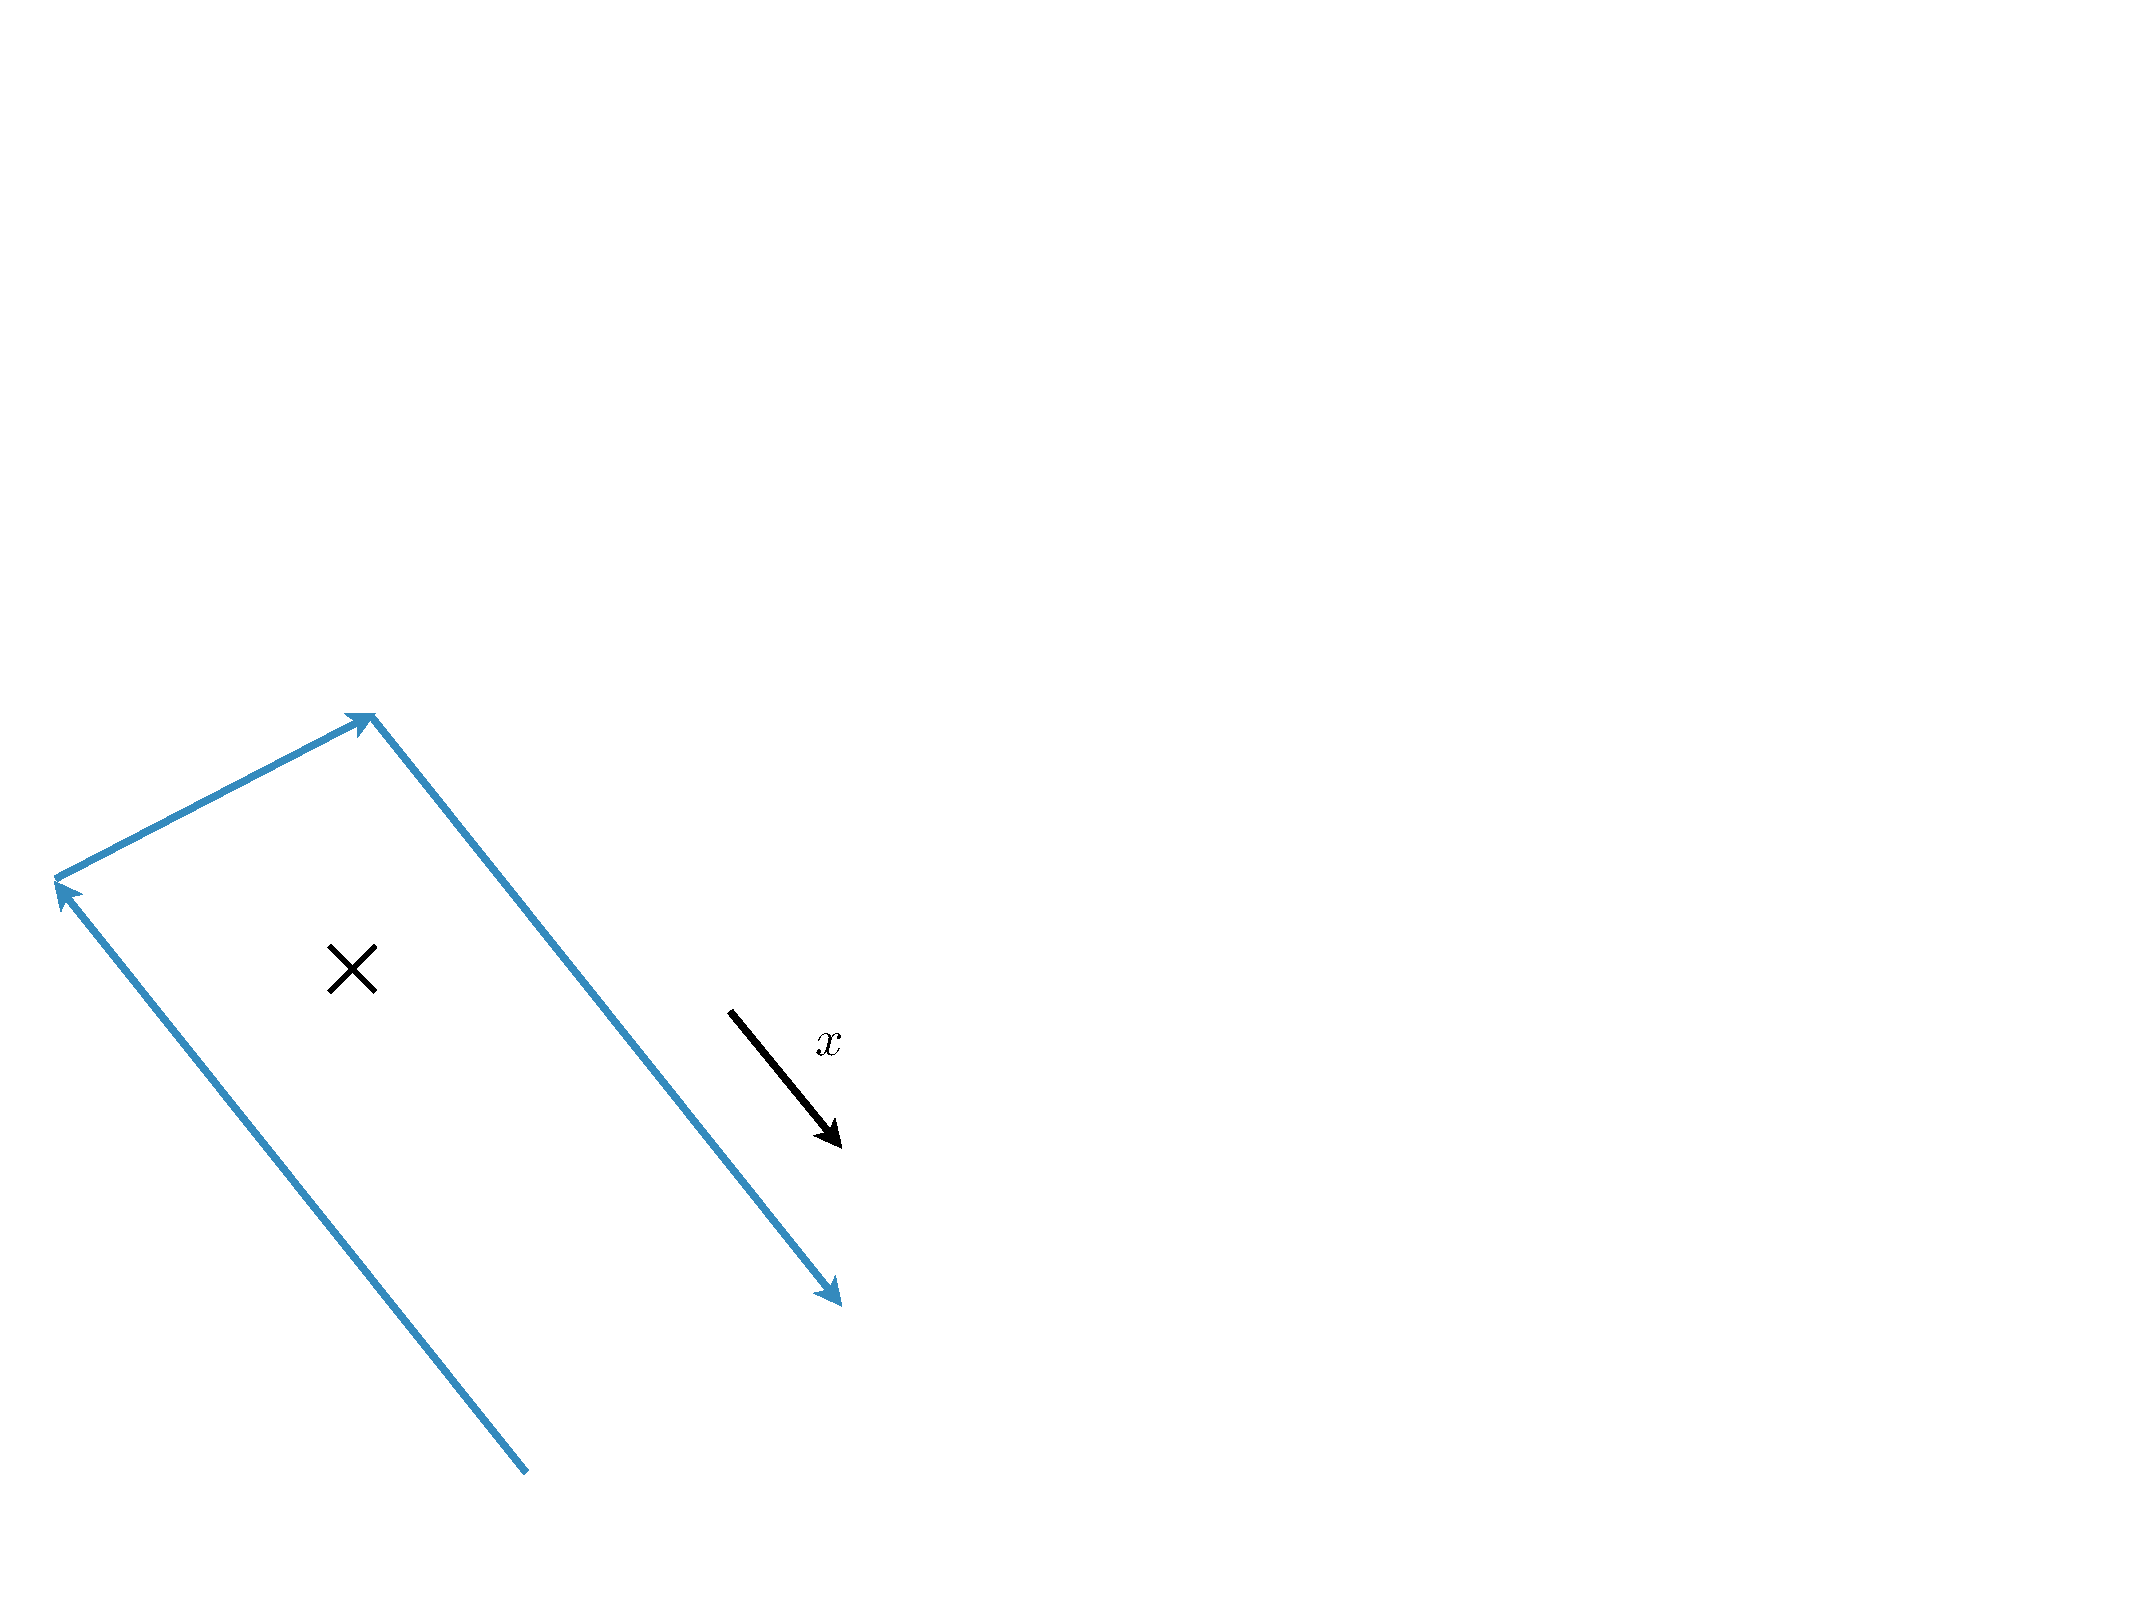
\includegraphics[width=2in]{figs/horseshoevortex}
\caption{}
\label{fig:horseshoevortex}
\end{figure}

\begin{figure}[htbp]
\centering
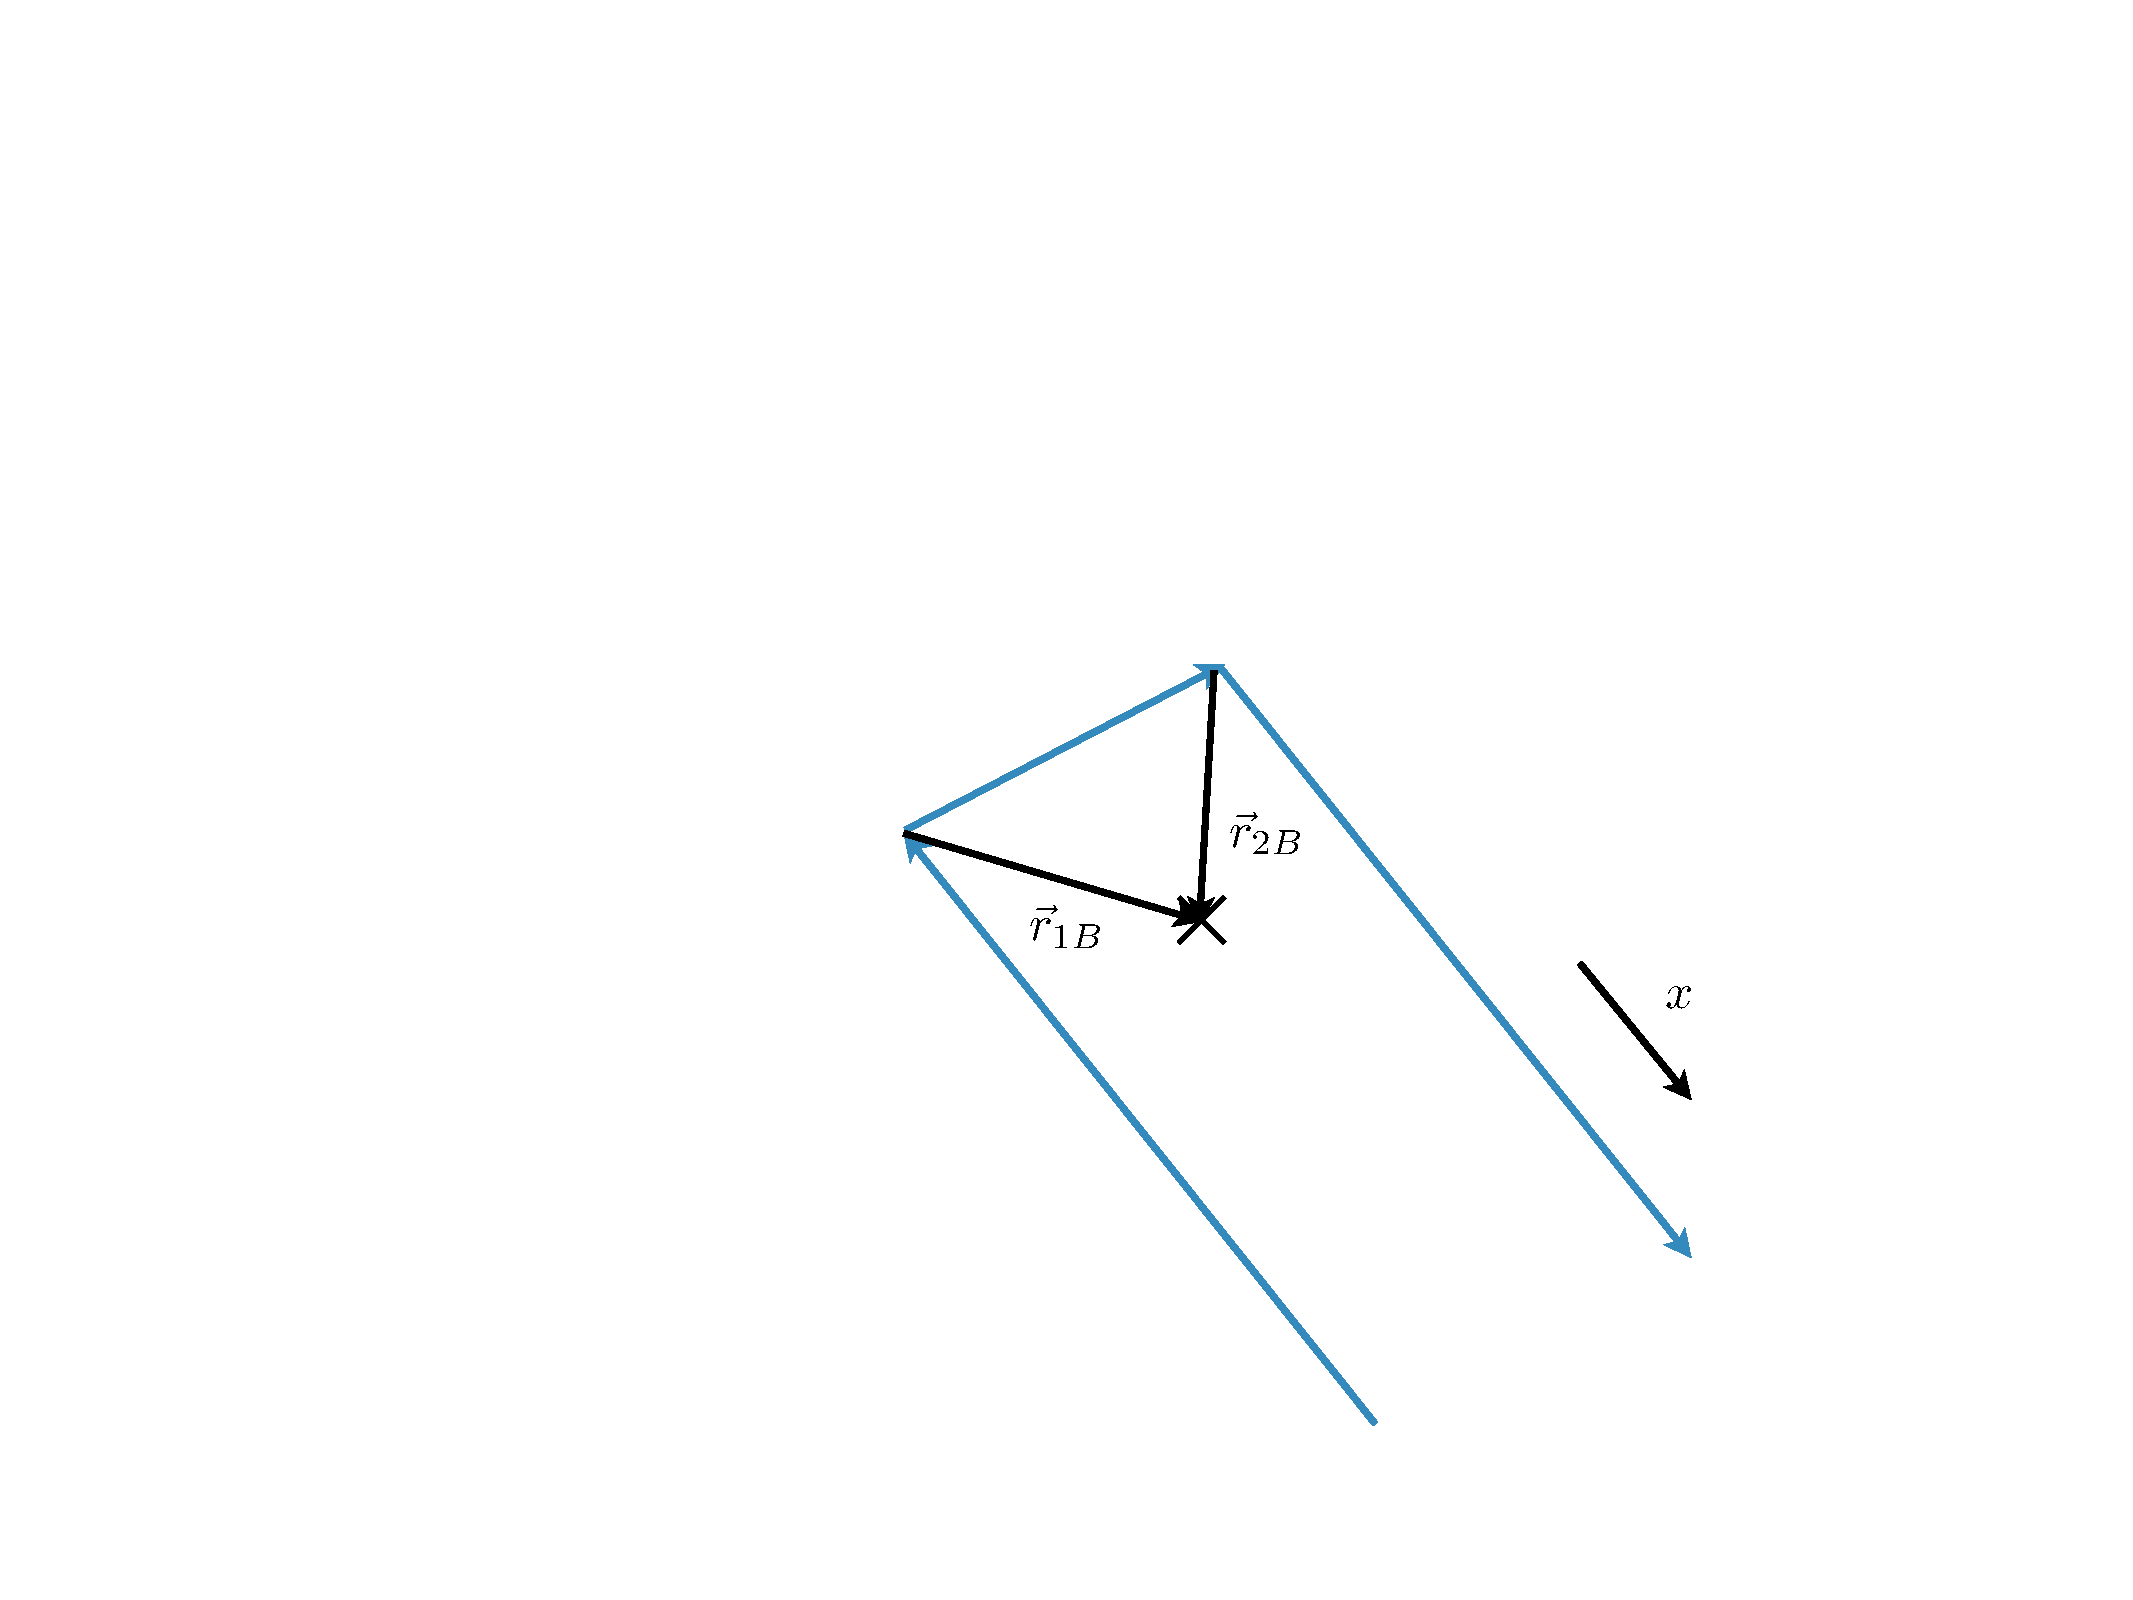
\includegraphics[width=2in]{figs/boundvortex}
\caption{}
\label{fig:boundvortex}
\end{figure}

The bound vortex uses all the terms of the formula. We use subscript $B$ to denote the vectors shown in \cref{fig:boundvortex}.
\begin{equation}
\vec{V}_{\theta B} = \frac{\Gamma}{4 \pi} \frac{\vec{r}_{1B} \times \vec{r}_{2B}}{(|\vec{r}_{1B}||\vec{r}_{2B}| + \vec{r}_{1B} \cdot \vec{r}_{2B})} \left(\frac{1}{|\vec{r_{1B}}|} + \frac{1}{|\vec{r_{2B}}|} \right)
\end{equation}

\begin{figure}[htbp]
\centering
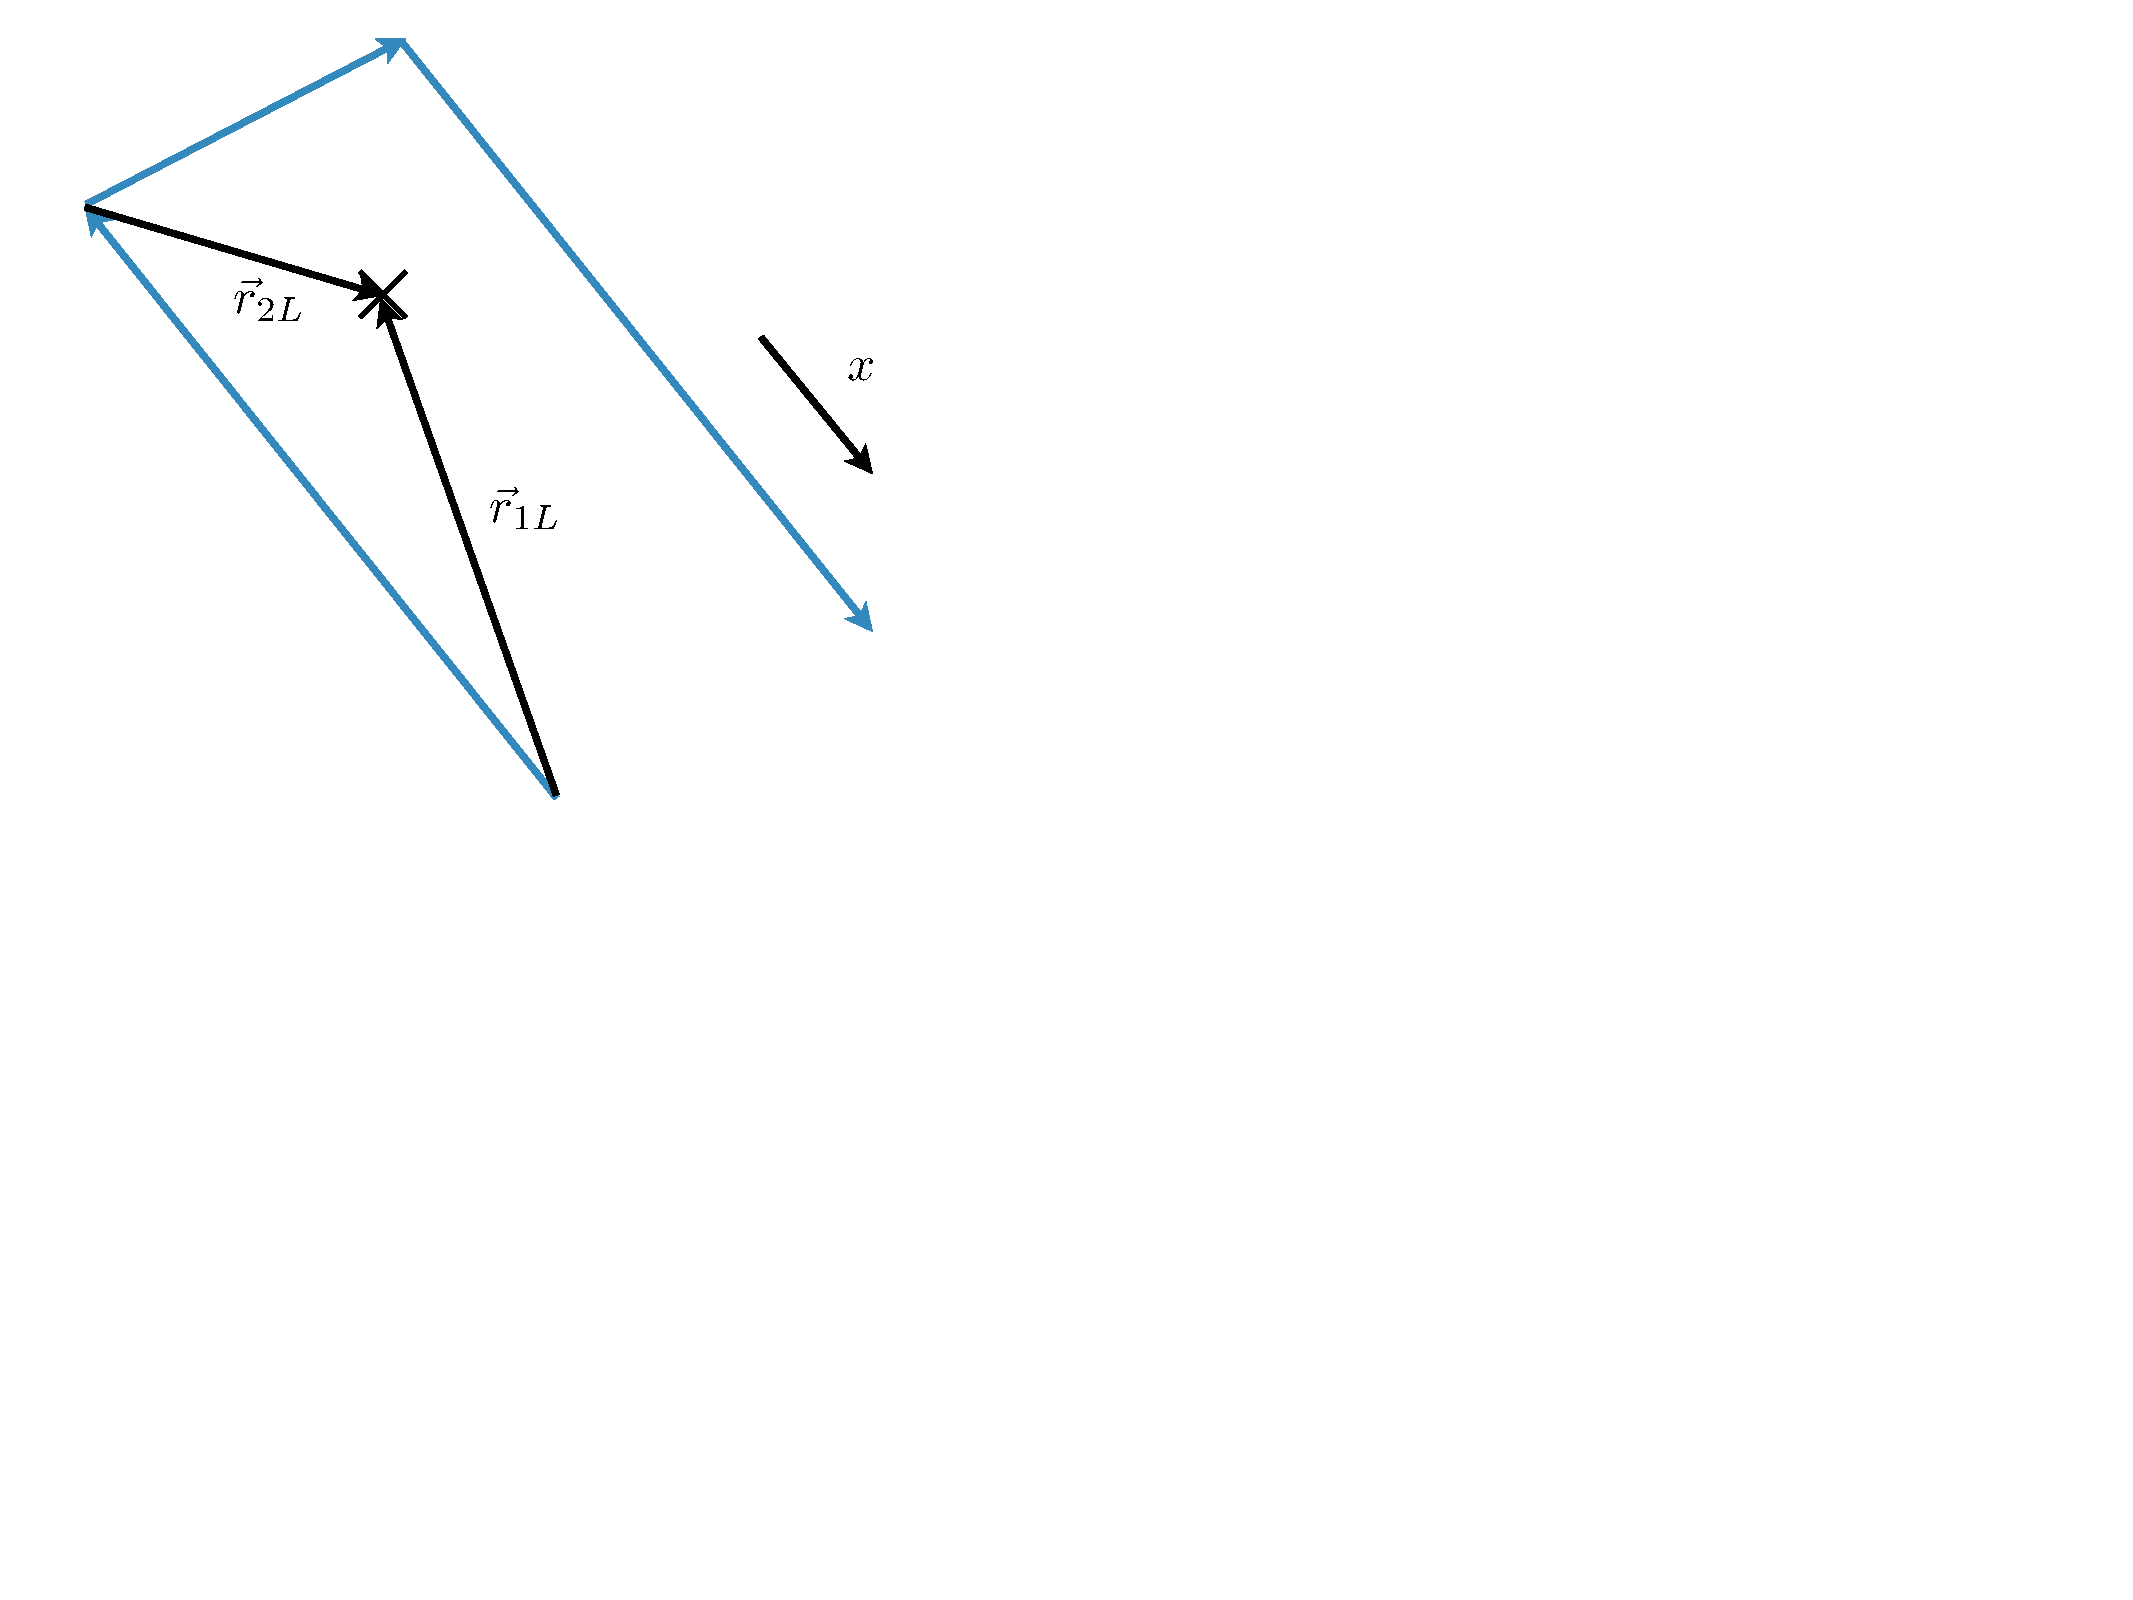
\includegraphics[width=2in]{figs/leftvortex}
\caption{}
\label{fig:leftvortex}
\end{figure}

For the left vortex (\cref{fig:leftvortex})
% \begin{equation}
% \vec{r}_{1L} = \lim_{\Delta x \rightarrow \infty} \Delta x \hat{x} + \Delta y \hat{y} + \Delta z \hat{z}
% \end{equation}
% and thus, 
we can see that as the end of the vortex goes to infinity:
\begin{align}
|\vec{r}_{1L}| &\rightarrow \infty\\
\frac{\vec{r}_{1L}}{|\vec{r}_{1L}|} &= -\hat{x}
\end{align}
If we divide the top and bottom of \cref{eq:segment} by $|\vec{r}_1|$ and let $|\vec{r}_1| \rightarrow \infty$ the expression simplifies (where we use $L$ to denote the left vortex.:
\begin{equation}
\vec{V}_{\theta L} = \frac{\Gamma}{4 \pi} \frac{-\hat{x} \times \vec{r}_{2L}}{(|\vec{r}_{2L}| - \hat{x} \cdot \vec{r}_{2L})} \left(\frac{1}{|\vec{r_{2L}}|} \right)
\end{equation}
But note that $\vec{r}_{2L} = \vec{r}_{1B}$, so we can rewrite this contribution as:
\begin{equation}
\vec{V}_{\theta L} = \frac{\Gamma}{4 \pi} \frac{\vec{r}_{1B} \times \hat{x}}{(|\vec{r}_{1B}| - \vec{r}_{1B} \cdot \hat{x})} \left(\frac{1}{|\vec{r_{1B}}|} \right)
\end{equation}

\begin{figure}[htbp]
\centering
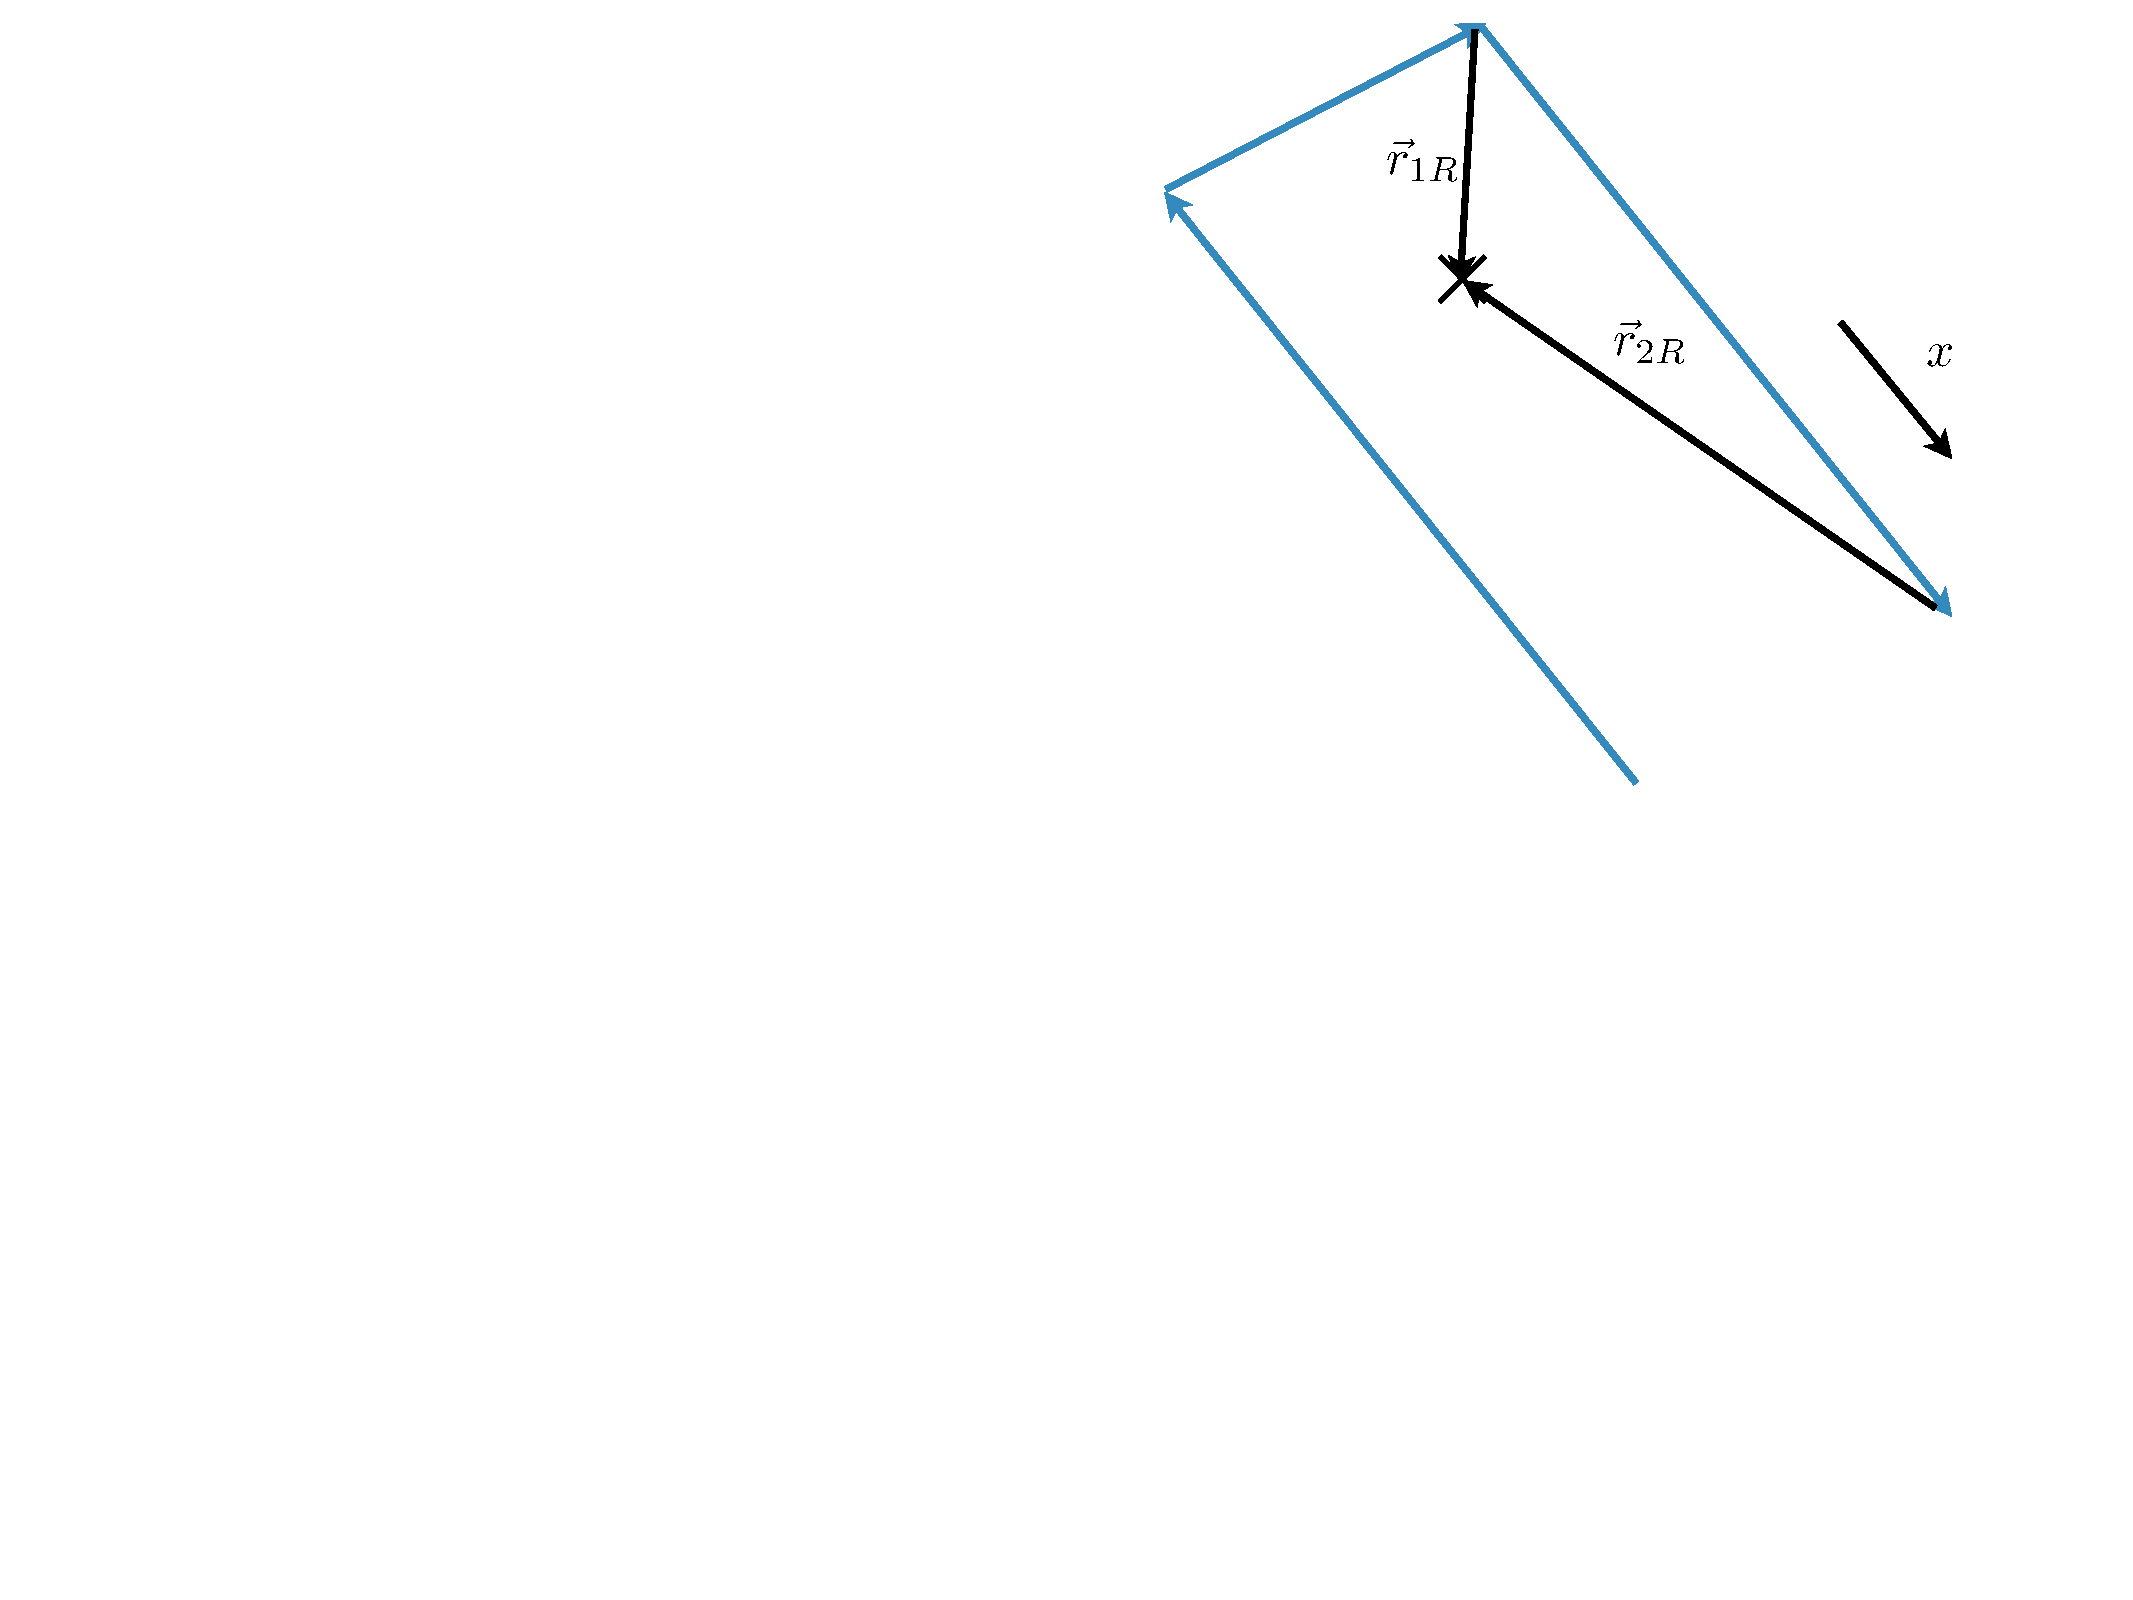
\includegraphics[width=2in]{figs/rightvortex}
\caption{}
\label{fig:rightvortex}
\end{figure}

For the right vortex (\cref{fig:rightvortex}) 
% \begin{equation}
% \vec{r}_2 = \lim_{\Delta x \rightarrow \infty} \Delta x \hat{x} + \Delta y \hat{y} + \Delta z \hat{z}
% \end{equation}
we see that as the vortex goes off to infinity:
\begin{align}
|\vec{r}_{2R}| &\rightarrow \infty\\
\frac{\vec{r}_{2R}}{|\vec{r}_{2R}|} &= -\hat{x}
\end{align}
If we divide the top and bottom of \cref{eq:segment} by $|\vec{r}_2|$ and let $|\vec{r}_2| \rightarrow \infty$ the expression simplifies (where we use $R$ to denote the left vortex):
\begin{equation}
\vec{V}_{\theta R} = \frac{\Gamma}{4 \pi} \frac{\vec{r}_{1R} \times -\hat{x}}{(|\vec{r}_{1R}| + \vec{r}_{1R} \cdot -\hat{x})} \left(\frac{1}{|\vec{r_{1R}}|} \right)
\end{equation}
But note that $\vec{r}_{1R} = \vec{r}_{2B}$, so we can rewrite this contribution as:
\begin{equation}
\vec{V}_{\theta R} = -\frac{\Gamma}{4 \pi} \frac{\vec{r}_{2B} \times \hat{x}}{(|\vec{r}_{2B}| - \vec{r}_{2B} \cdot \hat{x})} \left(\frac{1}{|\vec{r_{2B}}|} \right)
\end{equation}

Putting it all together (and dropping the $B$ subscript): the total induced velocity at some point $r$ measured relative to the bound vortex corners as seen in \cref{fig:boundvortex} is:
\begin{equation}
\vec{V} = 
\frac{\Gamma}{4 \pi} 
\left[
\frac{\vec{r}_{1} \times \vec{r}_{2}}{(|\vec{r}_{1}||\vec{r}_{2}| + \vec{r}_{1} \cdot \vec{r}_{2})} \left(\frac{1}{|\vec{r_{1}}|} + \frac{1}{|\vec{r_{2}}|} \right)
+
\frac{\vec{r}_{1} \times \hat{x}}{(|\vec{r}_{1}| - \vec{r}_{1} \cdot \hat{x})} \frac{1}{|\vec{r_{1}}|} 
-
\frac{\vec{r}_{2} \times \hat{x}}{(|\vec{r}_{2}| - \vec{r}_{2} \cdot \hat{x})} \frac{1}{|\vec{r_{2}}|} 
\right]
\end{equation}

Finally, we want the velocity for unit circulation and so 
\begin{equation}
\hat{V}_{ij} = 
\frac{1}{4 \pi} 
\left[
\frac{\vec{r}_{1} \times \vec{r}_{2}}{(|\vec{r}_{1}||\vec{r}_{2}| + \vec{r}_{1} \cdot \vec{r}_{2})} \left(\frac{1}{|\vec{r_{1}}|} + \frac{1}{|\vec{r_{2}}|} \right)
+
\frac{\vec{r}_{1} \times \hat{x}}{(|\vec{r}_{1}| - r_{1x})} \frac{1}{|\vec{r_{1}}|} 
-
\frac{\vec{r}_{2} \times \hat{x}}{(|\vec{r}_{2}| - r_{2x} )} \frac{1}{|\vec{r_{2}}|} 
\right]
\label{eq:vhorseshoe}
\end{equation}
where each vector points from the corner of the horseshoe vortex at position j to control point i:
\begin{align}
\vec{r}_1 &= \vec{r}_{CPi} - \vec{r}_{j}\\
\vec{r}_2 &= \vec{r}_{CPi} - \vec{r}_{j+1}
\end{align}

\subsection{Symmetry}

If the aircraft is symmetric then it is more efficient to only solve for the circulation on half of the aircraft.  This reduces the size of the linear system in half.  Solving a dense linear system is approximately an $\mathcal{O}(n^3)$ operation, and the linear system solve is the main computational cost of the VLM, so if taking advantage of symmetry is possible it is generally worth doing.  This is straightforward in constructing the AIC matrix.  The only change is that each control point we need to add the influence of horseshoe vortex $i$ as well as its mirror image $-i$.  The vector $\vec{r}_{-i}$ is identical to $\vec{r}_{i}$ except that the sign of the y component is flipped (we are assuming symmetry about the x-z plane).

\section{Near-Field Forces and Moments}

With the exception of induced drag, which is most accurately computed in the farfield, all other forces and moments are computed in the near field using the Kutta-Joukowski theorem:
\begin{equation}
\vec F^\prime_i = \rho \vec V_i \times \vec \Gamma_i
\end{equation}
First, we must compute the local velocity vector at each bound vortex.  Like the boundary condition, this requires a sum of the the freestream velocity (translation), rotation, induced velocity and other external velocities.  
\begin{equation}
\vec V = \vec{V}_\infty - \vec{\Omega} \times \vec{r}_b + \vec{V}_{ind} + \vec{V}_{other}
\end{equation}
This time the induced velocity is not computed at the control points, but rather at the center of the bound vortex.  We can reuse \cref{eq:vhorseshoe}, but evaluated at the center of each bound vortex.  This eliminates the first term because the bound vortex does not induce any velocity on itself.  The velocity induced at the center of vortex i is
\begin{equation}
\vec{V}_{ind, i} = \sum \Gamma_j \hat{V}_{ij}
\end{equation}
The induced velocity per unit circulation, $\hat{V}_{ij}$, is computed using the following vectors.
\begin{align}
\vec{r}_1 &= {\vec r}_{i,mid} - \vec{r}_{j}\\
\vec{r}_2 &= {\vec r}_{i,mid} - \vec{r}_{j+1}
\end{align}
where ${\vec r}_{i,mid} = (\vec{r}_i + \vec{r}_{i+1})/2$.  


Using the Kutta-Joukowski theorem, where the force is constant across a panel results in a force for each panel of:
\begin{equation}
\vec F_i = \rho \vec V_i \times \vec \Gamma_i \Delta s_i
\end{equation}
where the direction of $\Gamma$ is defined by
\begin{equation}
\vec \Gamma_i \Delta s_i = \Gamma_i (\vec{r}_{i+1} - \vec{r}_{i})
\end{equation}
The total forces are then
\begin{align}
\vec{F} &= \sum_i \vec{F}_i\\
&= \sum_i \rho \Gamma_i \left(\sum_j (\Gamma_j \hat{V}_{ij} ) + \vec{V}_\infty - \vec{\Omega} \times \vec{r}_i + \vec{V}_{other, i}\right)\times  (\vec{r}_{i+1} - \vec{r}_{i})
\label{eq:forces}
\end{align}
The total moments are given by:
\begin{equation}
\vec M = \sum_i \vec r_{m, i} \times \vec{F}_i
\end{equation}
where $\vec r_{m, i}$ is the vector originating from some specified reference point (often the aircraft c.g.) and ending at the location of force $F_i$ (i.e., $\vec r_{m, i} = \vec r_{i, mid} - \vec r_{cg}$).

For convenience, we can also express these calculations as matrix vector products (help when deriving derivatives for the stability derivatives).  For example, the x-component of the force is given by:
\begin{equation}
F_x  = \Gamma^T C_x \Gamma + e_x^T \Gamma
\label{eq:forcematrixvector}
\end{equation}
where
\begin{align}
{C_x}_{ij} &= \rho \left(\hat{V}_{ij} \times (\vec{r}_{i+1} - \vec{r}_{i})\right)_x\\
{e_x}_{i} &= \rho \left((\vec{V}_\infty - \vec{\Omega} \times \vec{r}_i + \vec{V}_{other, i}) \times (\vec{r}_{i+1} - \vec{r}_{i})\right)_x
\end{align}

These forces and moments are in the body coordinate system.  However, as aerodynamicists, we generally care about forces in the wind axes (oriented with the freestream) because that is the coordinate system where lift and drag are defined.  The rotation from body axes to wind axes is accomplished by the following rotations:
\begin{equation}
\begin{bmatrix}
D\\
Y\\
L
\end{bmatrix}
= 
\begin{bmatrix}
\cos\beta & -\sin\beta & 0 \\
\sin\beta & \cos\beta & 0 \\
0 & 0 & 1\\
\end{bmatrix}
\begin{bmatrix}
\cos\alpha & 0 & \sin\alpha \\
0 & 1 & 0\\
-\sin\alpha & 0 & \cos\alpha \\
\end{bmatrix}
\begin{bmatrix}
F_x\\
F_y\\
F_z
\end{bmatrix}
\label{eq:forceswindframe}
\end{equation}
We rotate moments similarly, although for dynamics leaving them in the body-coordinate system in generally preferred.

% Computing lift is straightforward.  From the Kutta-Joukowski theorem we can compute the force per unit length as:
% This gives a force in the wind-aligned coordinate system.  Because the wing may have dihedral, only the vertical component contributes to lift.
% \begin{equation}
% L = \sum_i F^\prime_i \cos\phi_i \Delta s_i
% \end{equation}
% Or in terms of a vector-vector product:
% \begin{equation}
% L = LIC^T \Gamma
% \end{equation}
% where
% \begin{equation}
% LIC_i = \rho V_\infty (y_{i+1} - y_i)
% \end{equation}

% \subsection{Symmetry}
% If the wing is symmetric then we only need circulation over half of the lifting surface.  The summation is identical except we multiply by a factor of 2 to get the lift over the whole lifting surface.
% \begin{equation}
% LIC_i = 2 \rho V_\infty (y_{i+1} - y_i)
% \end{equation}


\section{Induced Drag Influence Coefficients (DIC)}

The induced drag is evaluated using a Trefftz plane analysis with a drag-free wake.  While a drag-free wake is nonphysical, a far-field analysis shows that the induced drag is the same\footnote{not exactly.  We do neglect a couple of terms, though a careful analysis of a variety of wing shapes shows those terms to be negligibly small, especially for the level of fidelity we are interested in with a VLM.} whether a force-free wake or a drag-free wake is used.  The latter is \emph{much} simpler and using our wind coordinate system, means that the wake simply projects straight back in the $+x_w$ direction (as used in the previous section).  The induced drag calculation then simply becomes a two-dimensional analysis computing the influence of the wake on itself.  The farfield analysis shows that the induced drag is (general, not specific to VLM:
\begin{equation}
D_i = \int \frac{\rho}{2} V_n \Gamma ds
\end{equation}
where the integral is performed across the wake trace, $\Gamma$ is the circulation shed at the trailing edge of the aircraft, equivalent to the potential jump across the wake, and $V_n$ is the normlwash (induced velocity normal to the wake).  For the VLM case, we have discretized spanwise panels and so the induced drag becomes a summation:
\begin{equation}
D_i = \frac{\rho}{2} \sum_i  {V_n}_i \Gamma_i \Delta s_i
\label{eq:idrag}
\end{equation}

\begin{figure}[htbp]
\centering
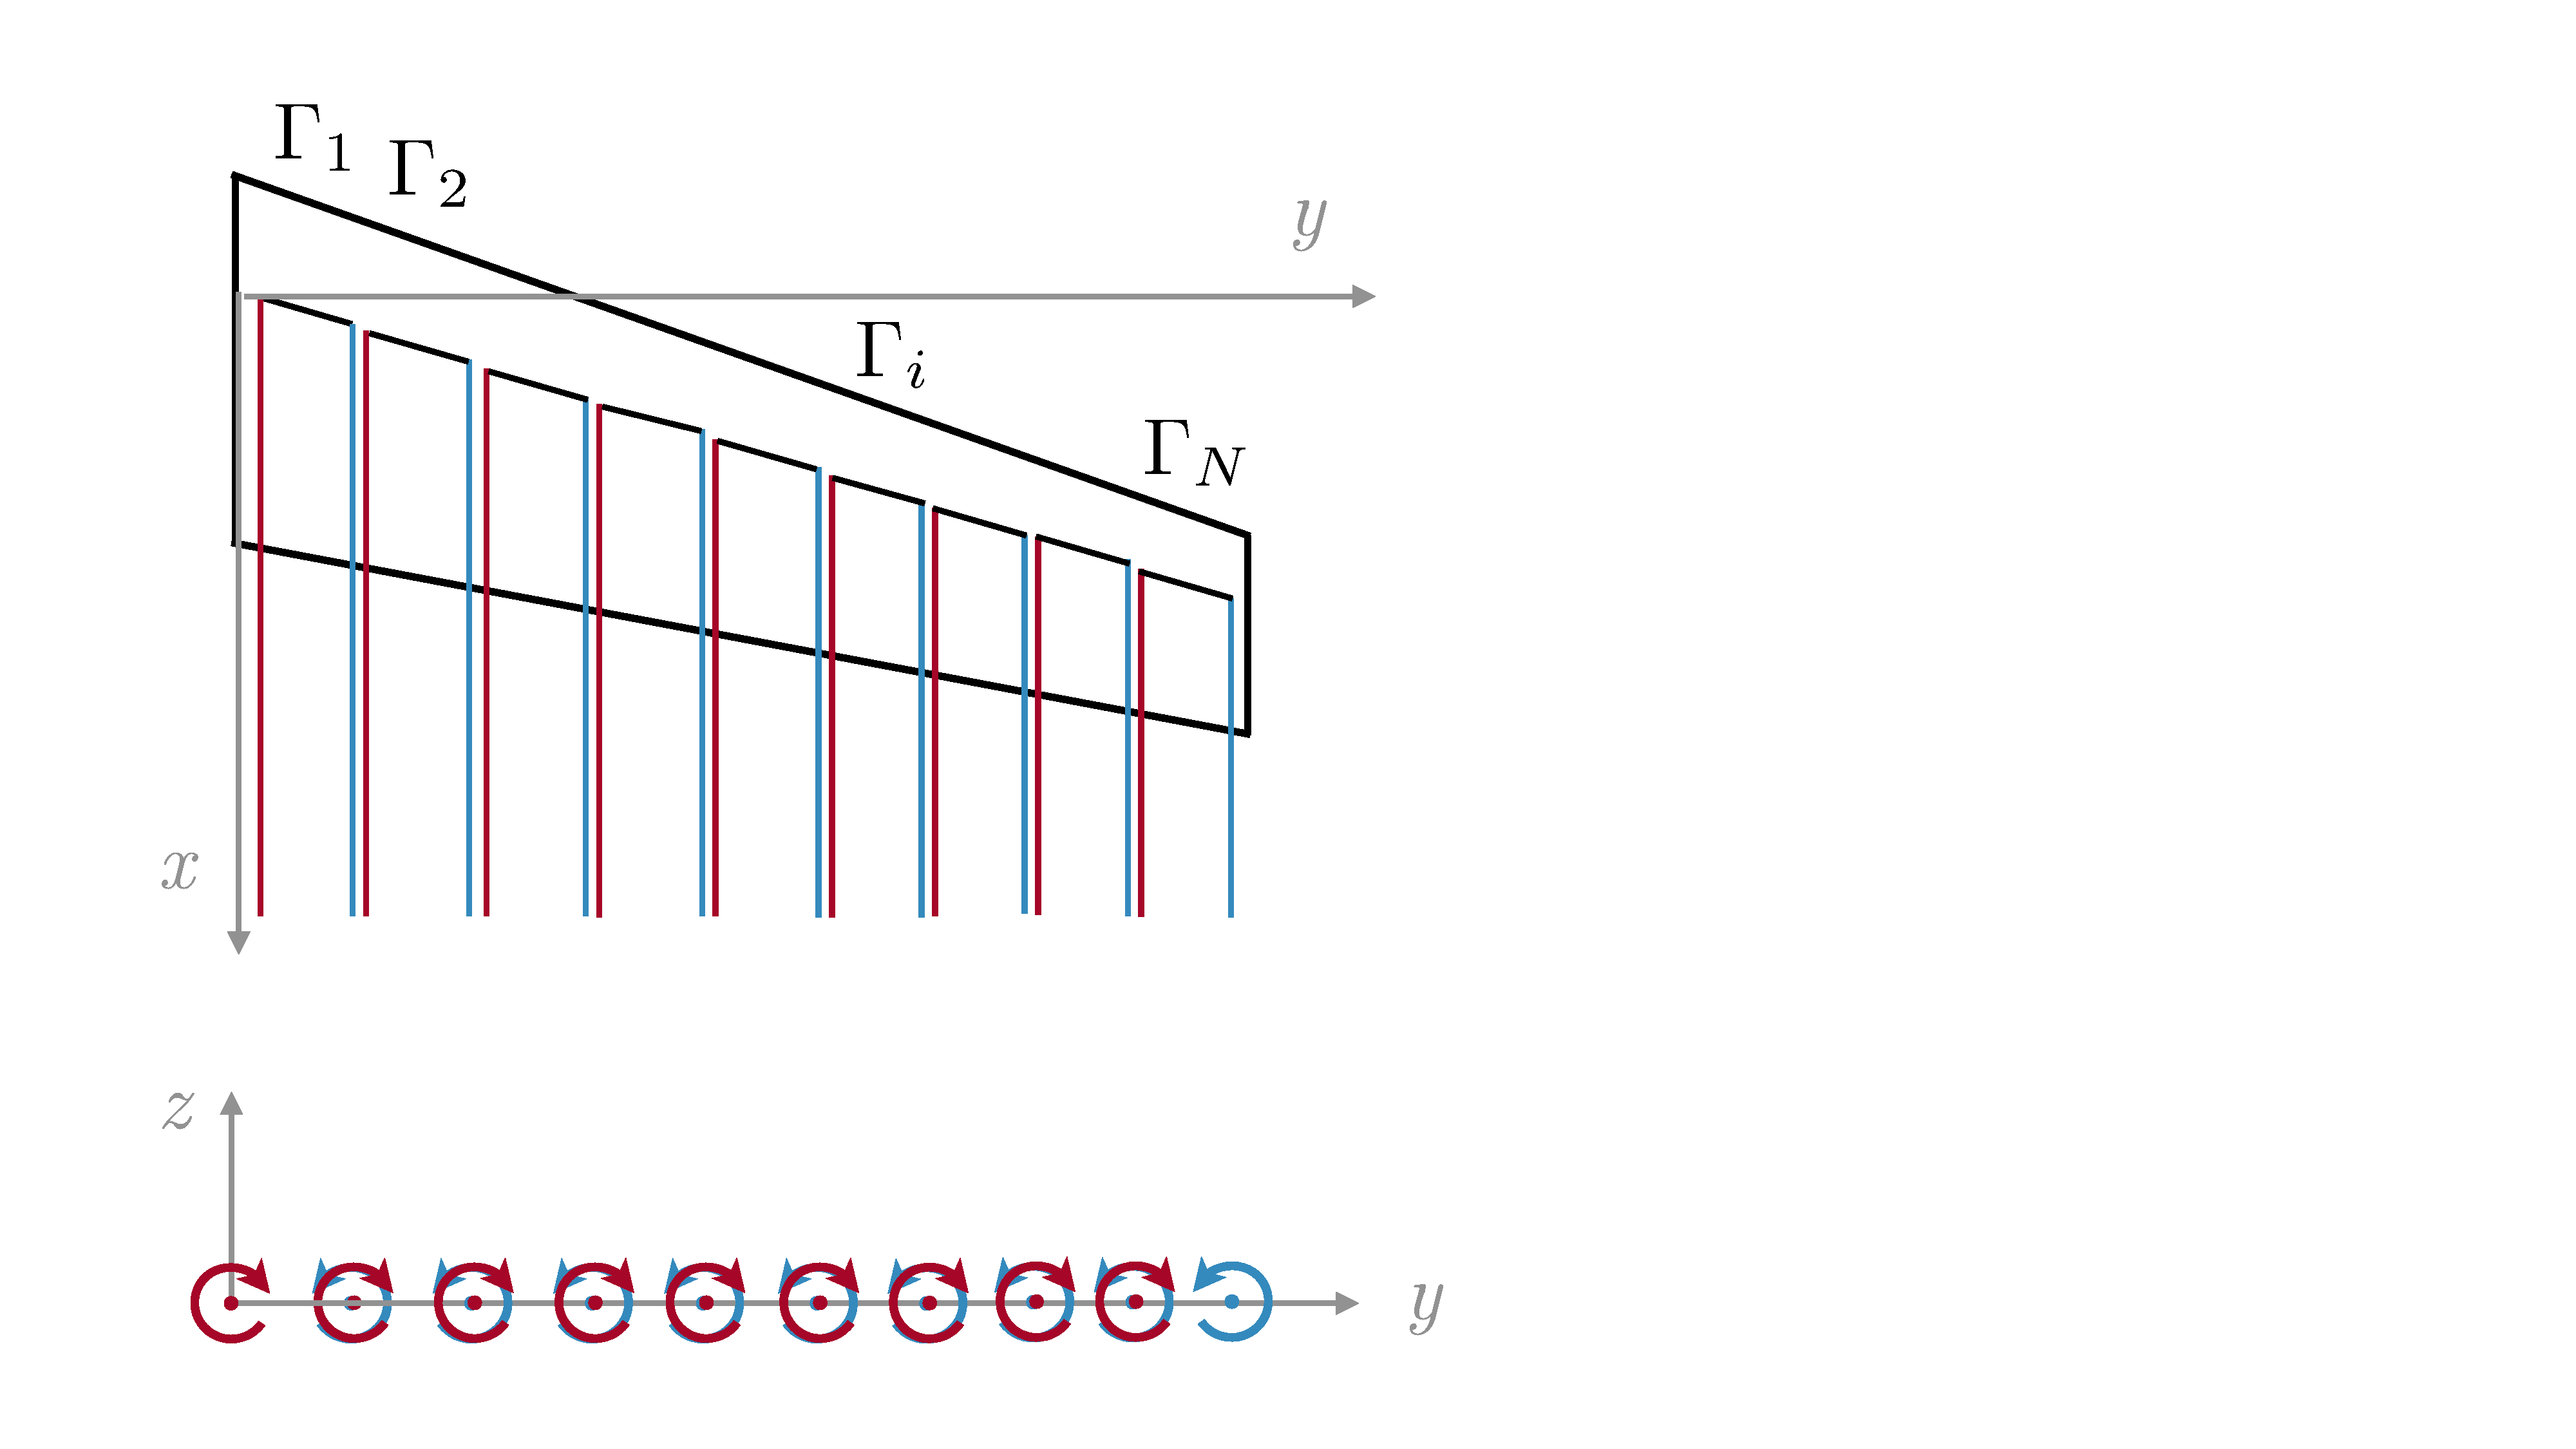
\includegraphics[width=3.0in]{figs/vlmwake}
\caption{}
\label{fig:vlmwake}
\end{figure}

Each panel sheds two vortices of opposite signs, that overlap with the neighboring vortices as shown in \cref{fig:vlmwake}.  These vortex strengths partially cancel, however it will be more convenient for our derivation (because we want to separate the geometry terms from the circulation terms) to consider the contributions one panel at a time.  For each panel we will need to include the contribution from the left and the right vortex.  The partial cancellation of vortex strengths will happen automatically as we sum panels, but not explicitly.  

\Cref{fig:induced} diagrams the analysis we need to perform.  Each panel has two counter rotating vortices as shown in the figure.  A given vortex from panel j induces a velocity on the center of  panel i. The center point of panel $i$ is given by:
\begin{align}
\bar{y}_i &= \frac{1}{2} (y_{i+1} + y_i)\\
\bar{z}_i &= \frac{1}{2} (z_{i+1} + z_i)\\
\end{align}
Each vortex $\Gamma_j$ induced a velocity given by:
The tangential velocity is given by:
\begin{equation}
\vec{V}_{\theta, i} = - \frac{\vec\Gamma_j \times \hat{r}_{ij}}{2 \pi |r_{ij}|} = - \frac{\vec\Gamma \times \vec{r_{ij}}}{2 \pi |r_{ij}|^2}
\end{equation}
The induced velocity $V_\theta$ is always perpendicular to $r_{ij}$, but we the component of velocity that is normal to panel $i$:
\begin{equation}
{V_n}_i = \vec{V}_{\theta, i} \cdot \hat{n}_i
\end{equation}

\begin{figure}[htbp]
\centering
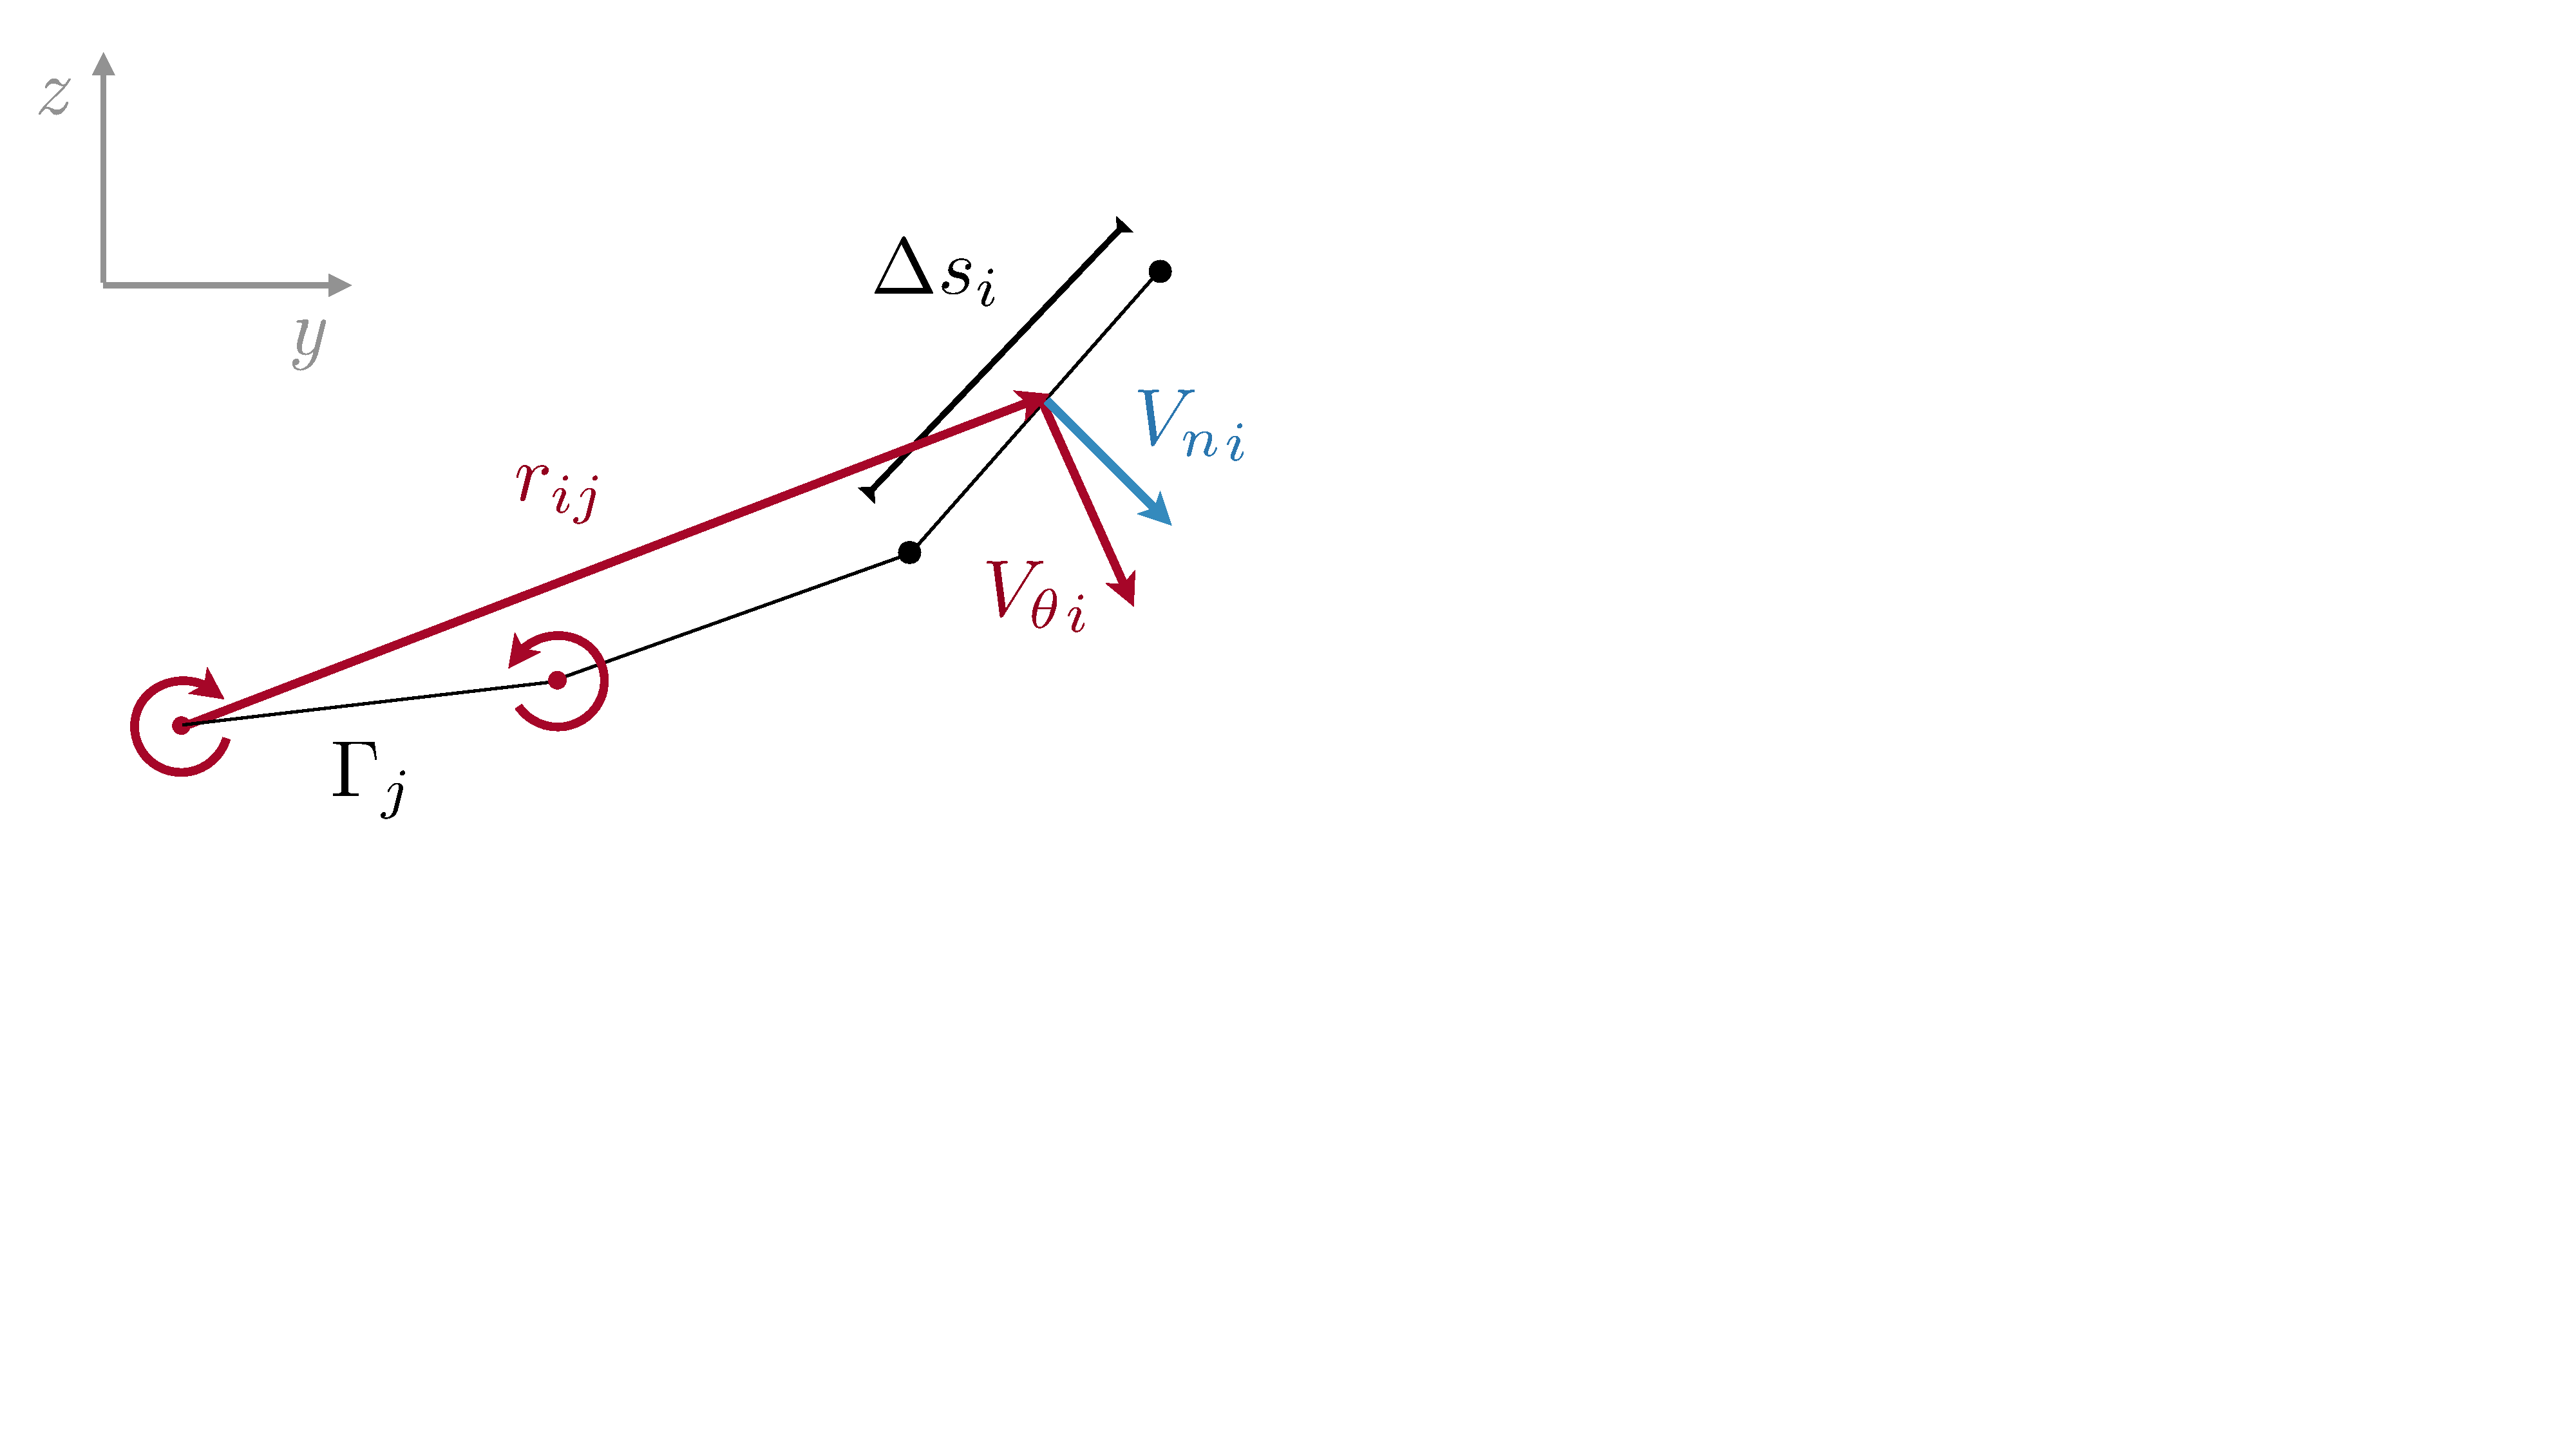
\includegraphics[width=2.25in]{figs/induced}
\caption{}
\label{fig:induced}
\end{figure}

The circulation is always aligned with the x-axis because it is a drag-free wake, and thus $r$ is always in the $y-z$ plane. Looking at just the contribution from the left vortex:
\begin{align}
    \vec\Gamma &= \Gamma \hat{x}\\
    \vec r &= (\bar{y}_i - y_j) \hat{y} + (\bar{z}_i - z_j) \hat{z}\\
    \vec\Gamma \times \vec{r} &= \Gamma_j (\bar{y}_i - y_j) \hat{z} - \Gamma_j (\bar{z}_i - z_j) \hat{y}\\
    \hat{n}_i &= \sin\phi_i \hat{y} - \cos\phi_i \hat{z}\\
    \hat{n}_i \Delta s_i &= (z_{i+1} - z_i) \hat{y} - (y_{i+1} - y_i) \hat{z}\\
    (\vec\Gamma \times \vec{r}) \cdot (\hat{n}_i \Delta s_i) &= - \Gamma_j (\bar{z}_i - z_j)(z_{i+1} - z_i) - \Gamma_j (\bar{y}_i - y_j)(y_{i+1} - y_i)\\
    {V_n}_{iL} \Delta s_i &= \frac{\Gamma_j (\bar{z}_i - z_j)(z_{i+1} - z_i) + \Gamma_j (\bar{y}_i - y_j)(y_{i+1} - y_i)}{2 \pi [(\bar{y}_i - y_j)^2 + (\bar{z}_i - z_j)^2]}
\end{align}
Adding the right vortex, and the summing up over all $j$ panels results in 
\begin{equation}
{V_n}_i \Delta s_i = \sum_{j=1}^N \frac{\Gamma_j}{2\pi} \left( k_{i,j} - k_{i, j+1}\right)
\end{equation}
where
\begin{equation}
k_{i,j} = \frac{(\bar z_i - z_j) (z_{i+1} - z_i) + (\bar y_i - y_j) (y_{i+1} - y_i)}{(\bar y_i - y_j)^2 + (\bar z_i - z_j)^2} 
\end{equation}
We can substitute this into the induced drag calculation \cref{eq:idrag} to get:
\begin{equation}
D_i = \frac{\rho}{2} \sum_i \Gamma_i \sum_{j=1}^N \frac{\Gamma_j}{2\pi} \left( k_{i,j} - k_{i, j+1}\right)
\end{equation}

This can be conveniently expressed in a quadratic form:
\begin{equation}
D_i = \Gamma^T [DIC] \Gamma
\end{equation}
where the induced drag coefficient matrix is given by:
\begin{equation}
DIC_{ij} = \frac{\rho}{4\pi} \left(k_{i,j} - k_{i, j+1}\right)
\end{equation}

\subsection{Symmetry}

If the wing and circulation distribution is symmetric, then the induced drag only requires a sum on half of the wing (multiplied by 2):
\begin{equation}
D_{ind} = \rho_\infty \sum_{i=1}^N {V_n}_i \Gamma_i  \Delta s_i
\end{equation}


\begin{figure}[htbp]
\centering
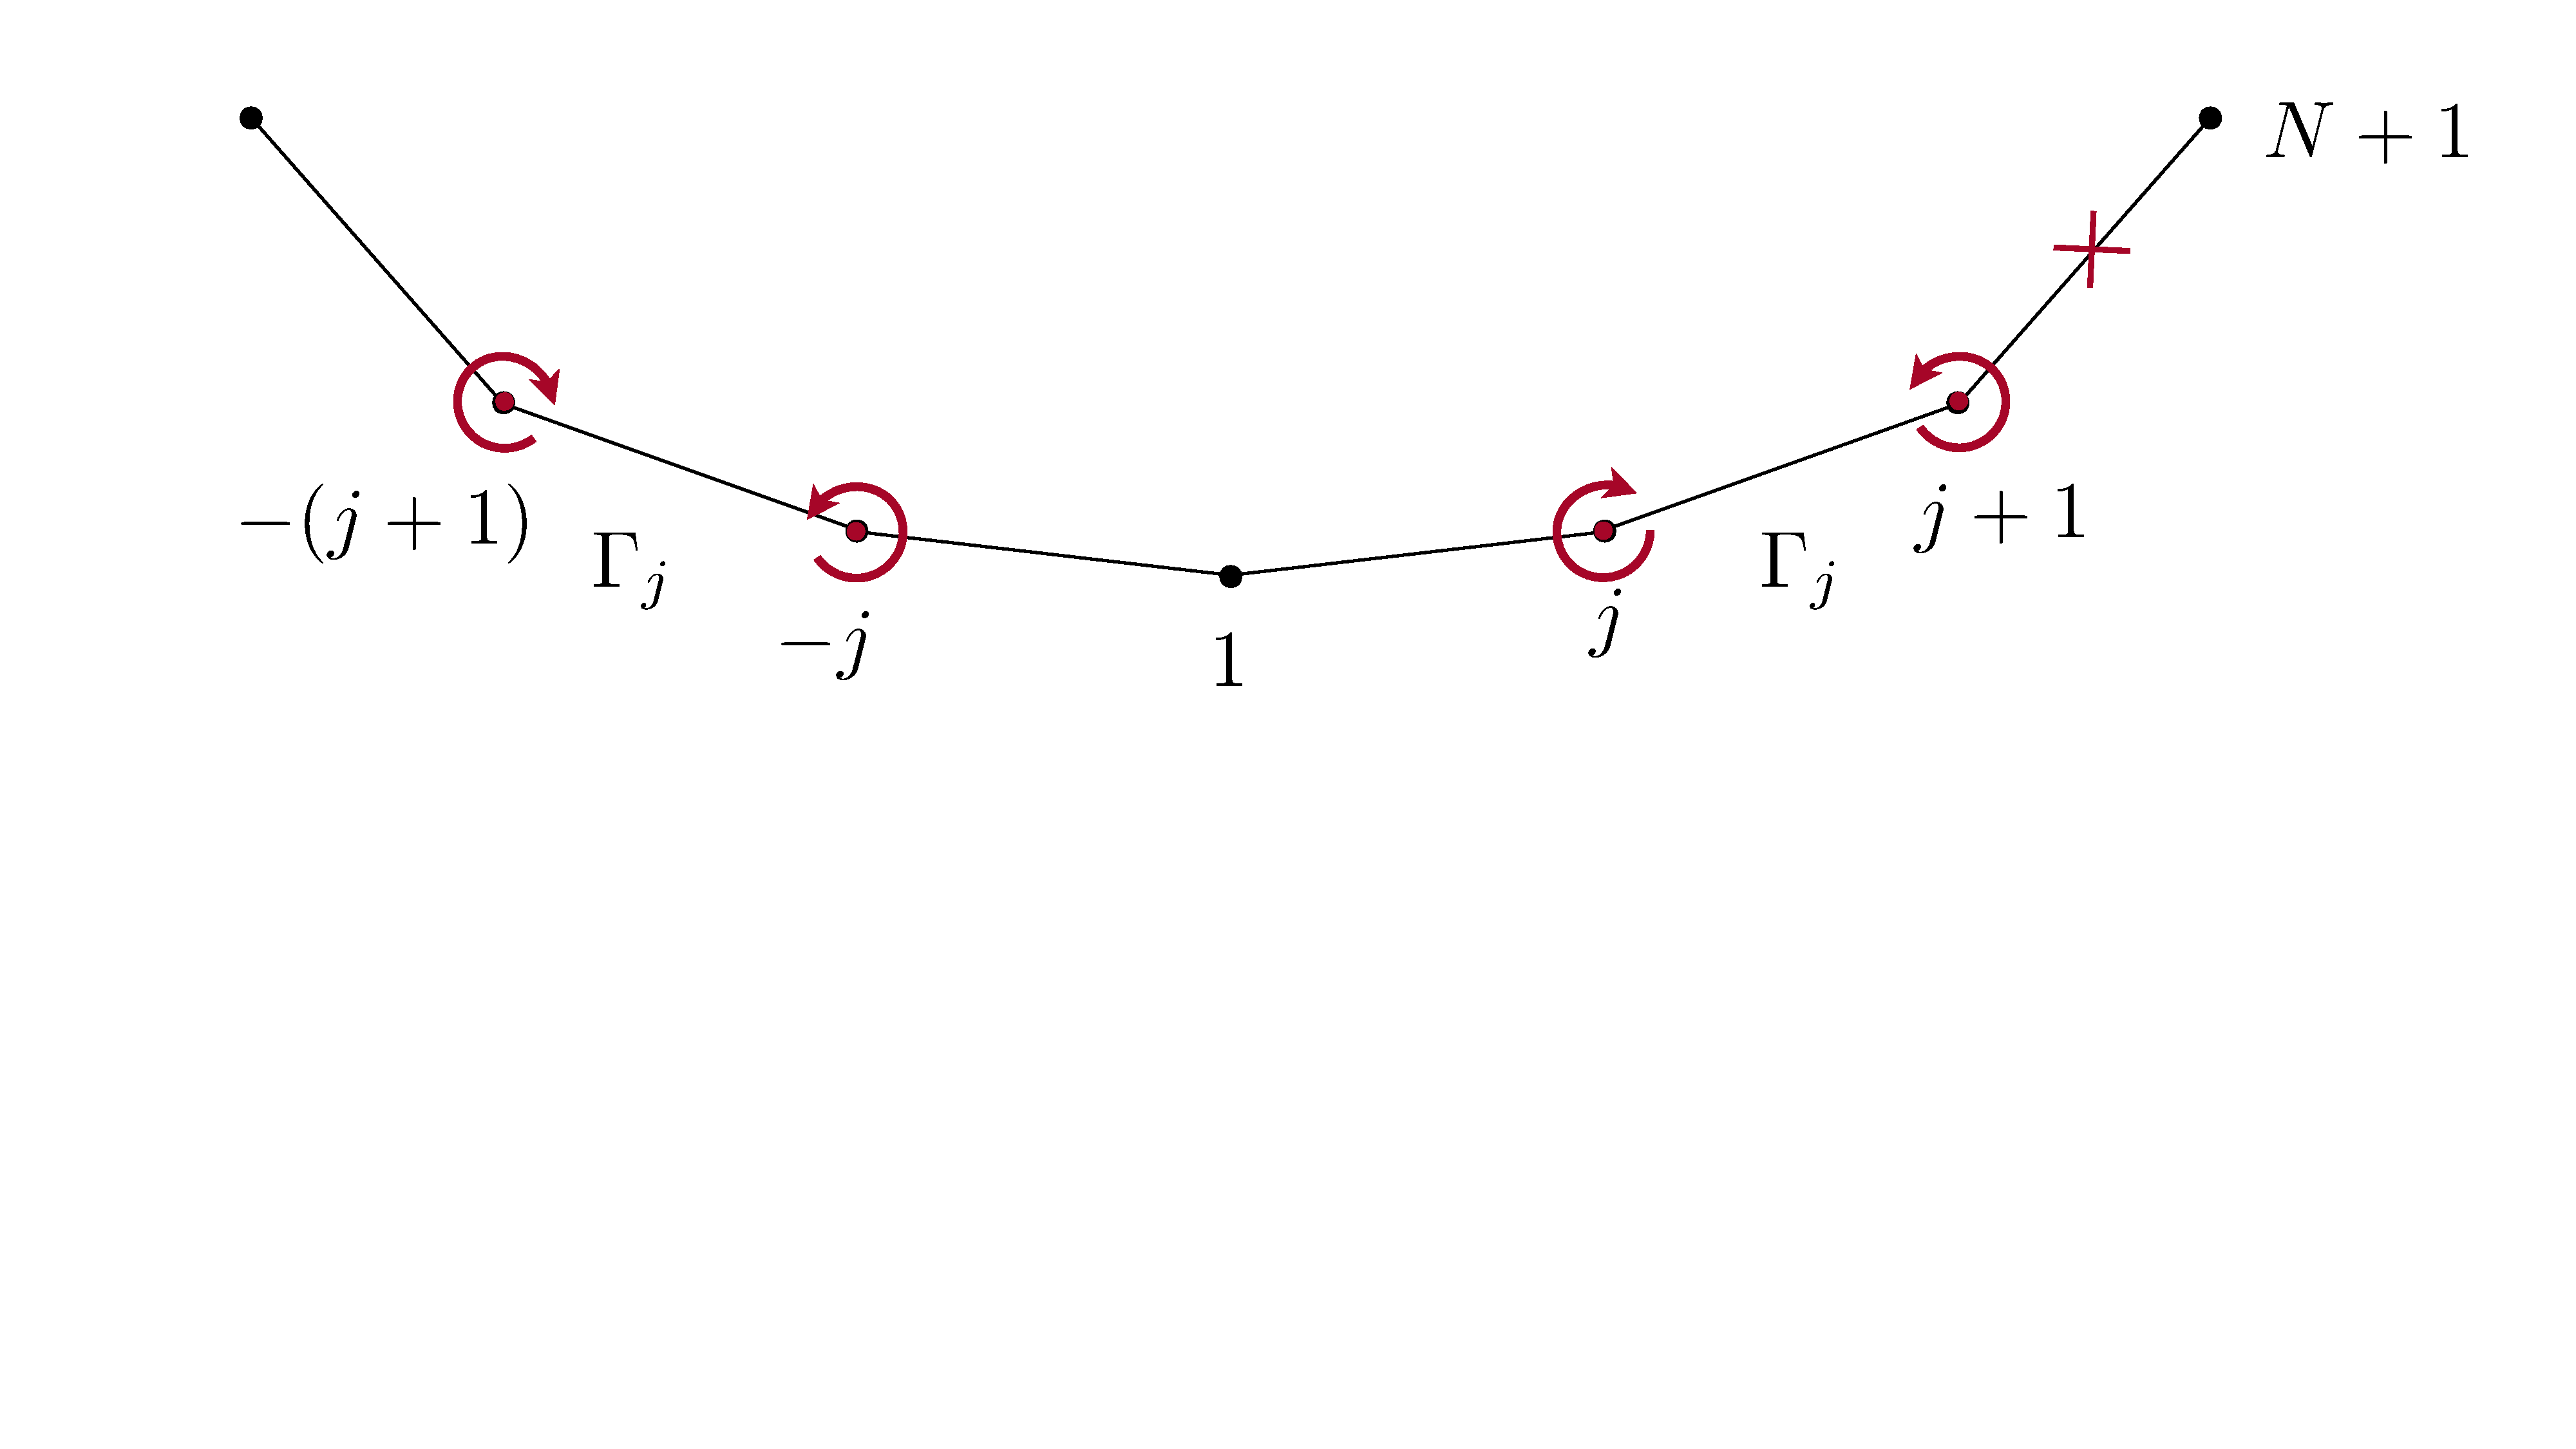
\includegraphics[width=3.5in]{figs/induced2}
\caption{}
\label{fig:induced2}
\end{figure}

When calculating the induced velocity at panel $i$ we should add not only the contribution from $\Gamma_j$ on the same side of the wing, but the contribution from $\Gamma_j$ on the opposite side of the wing as depicted in \cref{fig:induced2}.  The resulting normalwash is:
\begin{equation}
{V_n}_i \Delta s_i = \sum_{j=1}^N 
\frac{\Gamma_j}{2\pi} \left( 
k_{i,j} - k_{i, j+1} - k_{i, -j} + k_{i, -(j+1)}
\right)
\end{equation}
where
\begin{equation}
k_{i,\pm j} = \frac{(\bar z_i - z_j) (z_{i+1} - z_i) + (\bar y_i \mp y_j) (y_{i+1} - y_i)}{(\bar y_i \mp y_j)^2 + (\bar z_i - z_j)^2} 
\end{equation}
This leads to a DIC matrix of the following form:
\begin{equation}
DIC_{ij} = \frac{\rho_\infty}{2\pi} \left(k_{i,j} - k_{i, j+1} - k_{i, -j} + k_{i, -(j+1)}
\right)
\end{equation}



% Using our expression for the normalwash:
% \begin{equation}
% D_{ind} = \rho_\infty \sum_{i=1}^N \Gamma_i \sum_{j=1}^N 
% \frac{\Gamma_j}{2\pi} \left( 
% k_{i,j} - k_{i, j+1} - k_{i, -j} + k_{i, -(j+1)}
% \right)
% \end{equation}


\section{Stability Derivatives}

Let's start with derivatives with respect to angle of attack and sideslip.  From \cref{eq:Vinf} we can find derivatives for the freestream:
\begin{align}
\frac{d\vec{V}_{\infty}}{d\alpha} &= V_\infty
    \begin{bmatrix}
    -\sin\alpha\cos\beta\\
    0\\
    \cos\alpha\cos\beta
    \end{bmatrix}
% \frac{d\vec{V}_{\infty}}{d\beta} &= V_\infty
%     \begin{bmatrix}
%     -\cos\alpha\sin\beta\\
%     -\cos\beta\\
%     -\sin\alpha\sin\beta
%     \end{bmatrix}\\
\end{align}
The right hand side vector $b$ in \cref{eq:rhs} is given by:
\begin{equation}
b_i = - (\vec{V}_\infty - \vec{\Omega} \times \vec{r}_i +  \vec{V}_{other, i}) \cdot \hat{n}_{i}
\end{equation}
Thus:
\begin{equation}
\frac{d b_i}{d \alpha} = - \frac{d\vec{V}_{\infty}}{d\alpha} \cdot \hat{n}_i
\end{equation}
The circulation is solved as in \cref{eq:linearsystem} and so the derivative of the circulation is solved as:
\begin{equation}
 \frac{d \Gamma}{d \alpha} = [AIC]^{-1} \frac{d b}{d \alpha}
\end{equation}
where for computational efficiency we perform a linear system solve and not a matrix inversion.  The velocity at each panel center is given by the term in parenthesis in \cref{eq:forces}, and its derivative is:
\begin{equation}
\frac{d \vec{V}_i}{d \alpha} = \sum_j ( \frac{d \Gamma_j}{d \alpha}\hat{V}_{ij})+ \frac{d \vec{V}_\infty}{d \alpha}
\end{equation}
The derivative of the forces is then:
\begin{equation}
\frac{d \vec{F}}{d \alpha} = \rho \sum_i \left[\left(\Gamma_i \frac{d \vec{V}_i}{d \alpha} +  \frac{d \Gamma_i}{d\alpha} V_i \right) \times (\vec{r}_{i+1} - \vec{r}_{i}) \right]
\end{equation}
and the moments:
\begin{equation}
\frac{d\vec M}{d\alpha} = \sum_i \vec r_{m, i} \times \frac{d \vec{F}_i}{d\alpha}
\end{equation}
% \begin{align}
% \vec{F} &= \sum_i \vec{F}_i\\
% &= \sum_i \rho \Gamma_i \left(\sum_j (\Gamma_j \hat{V}_{ij} ) + \vec{V}_\infty - \vec{\Omega} \times \vec{r}_i + \vec{V}_{other, i}\right)\times  (\vec{r}_{i+1} - \vec{r}_{i})
% \end{align}
% \begin{equation}
% \frac{d F_x}{d\alpha} = \Gamma^T (C_x^T + C_x) \frac{d \Gamma}{d \alpha} + e_x^T \frac{d \Gamma}{d \alpha} + \Gamma^T \frac{d e_x}{d \alpha}
% \end{equation}
% where
% \begin{equation}
% \frac{d e_x}{d \alpha} =  \rho \left(\frac{d\vec{V}_{\infty}}{d\alpha} \times (\vec{r}_{i+1} - \vec{r}_{i}) \right)_x
% \end{equation}
% and similarly for the y and z components of the force.  
The forces in the wind frame are given by \cref{eq:forceswindframe} and so
\begin{equation}
\frac{d }{d\alpha} \begin{bmatrix}
D\\
Y\\
L
\end{bmatrix} 
= R_\beta R_\alpha \frac{d }{d\alpha} 
\begin{bmatrix}
F_x\\
F_y\\
F_z
\end{bmatrix}
+ 
R_\beta \frac{d R_\alpha}{d\alpha} 
\begin{bmatrix}
F_x\\
F_y\\
F_z
\end{bmatrix}
\end{equation}
where $R_\beta$ and $R_\alpha$ are the rotation matrices and
\begin{equation}
\frac{d R_\alpha}{d\alpha}  =
\begin{bmatrix}
-\sin\alpha & 0 & \cos\alpha \\
0 & 0 & 0\\
-\cos\alpha & 0 & -\sin\alpha \\
\end{bmatrix}
\end{equation}
Finally, the lift and drag coefficients differ only by a constant term and so:
\begin{equation}
\frac{d }{d\alpha} 
\begin{bmatrix}
C_D\\
C_Y\\
C_L
\end{bmatrix} 
=
\frac{1}{q_\infty S_{ref}}
\frac{d }{d\alpha} 
\begin{bmatrix}
D\\
Y\\
L
\end{bmatrix} 
\end{equation}
This process is the same for sideslip, and rotation.  The derivative for $p, q, r$ are easily found for the total velocity by expanding the cross product.
\begin{equation}
- \Omega \times r = 
\begin{bmatrix}
- q r_z + r r_y\\
p r_z - r r_x\\
- p r_y + q r_x
\end{bmatrix}
\end{equation}





\end{document}
